%% The '3p' and 'times' class options of elsarticle are used for Elsevier CRC
%% The 'procedia' option causes ecrc to approximate to the Word template
\documentclass[3p,times,procedia]{elsarticle}
\flushbottom

%% The `ecrc' package must be called to make the CRC functionality available
\usepackage{ecrc}

\usepackage{moreverb,url}

\usepackage[colorlinks,bookmarksopen,bookmarksnumbered,citecolor=red,urlcolor=red]{hyperref}

\usepackage{chngpage}

\newcommand\BibTeX{{\rmfamily B\kern-.05em \textsc{i\kern-.025em b}\kern-.08em
T\kern-.1667em\lower.7ex\hbox{E}\kern-.125emX}}

\def\volumeyear{2017}


\usepackage[utf8]{inputenc}
\usepackage[T1]{fontenc}

%%%%%
% variable to include comments or not in the compilation ; set to 1 to include
%\def \draft {1}
\def \draft {0}



\usepackage{xparse}
\usepackage{ifthen}

\DeclareDocumentCommand{\comment}{o m o o o o}
{\ifthenelse{\draft=1}{
  \IfValueT{#1}{
      \textcolor{red}{\textbf{C (#1) : }#2}
      \IfValueT{#3}{\textcolor{blue}{\textbf{A1 : }#3}}
      \IfValueT{#4}{\textcolor{ForestGreen}{\textbf{A2 : }#4}}
      \IfValueT{#5}{\textcolor{red!50!blue}{\textbf{A3 : }#5}}
      \IfValueT{#6}{\textcolor{Aquamarine}{\textbf{A4 : }#6}}
    }
    \IfNoValueT{#1}{
      \textcolor{red}{\textbf{C : }#2}
      \IfValueT{#3}{\textcolor{blue}{\textbf{A1 : }#3}}
      \IfValueT{#4}{\textcolor{ForestGreen}{\textbf{A2 : }#4}}
      \IfValueT{#5}{\textcolor{red!50!blue}{\textbf{A3 : }#5}}
      \IfValueT{#6}{\textcolor{Aquamarine}{\textbf{A4 : }#6}}
    }
 }{}
}




% todo
%\newcommand{\todo}[1]{
%\ifthenelse{\draft=1}{\textcolor{red!50!blue}{\textbf{TODO : \textit{#1}}}}{}
%}
\DeclareDocumentCommand{\todo}{o m}{
  \ifthenelse{\draft=1}{
    \IfValueT{#1}{\textcolor{red!50!blue}{\textbf{TODO (#1) : \textit{#2}}}}
    \IfNoValueT{#1}{\textcolor{red!50!blue}{\textbf{TODO : \textit{#2}}}}
  }{}
}

%\date{}
%\renewcommand\abstractname{\fontsize{14pt}{0}\textbf{Abstract}\selectfont}

%\usepackage[left=25mm, right=25mm, top=25mm, bottom=25mm, includehead=false, includefoot=false]{geometry}

%\usepackage{graphicx}
%\usepackage{url}
%\usepackage[round,semicolon]{natbib}  % Citation styles https://www.sharelatex.com/learn/Natbib_citation_styles
%\bibliographystyle{humannat}
%\renewcommand{\bibsection}{}
%\renewcommand{\bibhang}{\setlength{-1px}}


%\usepackage{authblk} % For author lists
%\renewcommand\Authfont{\fontsize{11}{1}\selectfont}
%\renewcommand\Affilfont{\fontsize{9}{1}\selectfont}

%\renewcommand*\footnoterule{}

\usepackage[table]{xcolor}
\usepackage[parfill]{parskip} % Line between paragraphs
\usepackage{amsmath}
%\pagenumbering{arabic} 

%\usepackage{sectsty}
%\allsectionsfont{\sffamily}

%\usepackage[pdftex]{hyperref} 
%\hypersetup{pdfborder={0 0 0} }


\usepackage[flushleft]{threeparttable}



%%%%%%%%%%%%%%%%%%%%%%%%%
%% -- from ecrc template
%%%%%%%%%%%%%%%%%%%%%%%%%


%% set the volume if you know. Otherwise `00'
\volume{00}

%% set the starting page if not 1
\firstpage{1}



\jid{}


\biboptions{authoryear}




\usepackage{soul}
\soulregister\cite7
\soulregister\citep7
\soulregister\ref7

%\usepackage[final]{changes}
\usepackage{changes}


\setaddedmarkup{\textcolor{black}{\hl{#1}}}
\setdeletedmarkup{\textcolor{red}{\sout{#1}}}

% add line number
\usepackage{lineno}
\linenumbers








%\runauth{Raimbault et al.}
\runauth{}

\begin{document}

% **************  TITLE AND AUTHOR INFORMATION **************


\begin{frontmatter}

\dochead{}

\title{Space Matters: extending sensitivity analysis to initial spatial conditions in geosimulation models
%Initial spatial conditions in simulation models: the missing leg of sensitivity analyses?
}

\author[a,b]{Juste Raimbault\corref{cor1}}
\author[c,d]{Cl{\' e}mentine Cottineau}
\author[e]{Marion Le Texier}
\author[f]{Florent Le N{\' e}chet}
\author[a]{Romain Reuillon}


\address[a]{UPS CNRS 3611 ISC-PIF, Paris, France}
\address[b]{UMR CNRS 8504 G{\'e}ographie-cit{\'e}s, Paris, France}
\address[c]{Centre for Advanced Spatial Analysis, University College London, UK}
\address[d]{UMR CNRS 8097 Centre Maurice Halbwachs, Paris, France}
\address[e]{UMR 6266 IDEES, Universit{\'e} de Rouen Normandie, France}
\address[f]{Université Paris-Est, Laboratoire Ville Mobilité Transport, Marne-la-Vallée, France}
%NB : mon affiliation "officielle" c'est : 
%Le Néchet, F., Université Paris-Est, Laboratoire Ville Mobilité Transport, UPEMLV : 5 boulevard Copernic, Cité Descartes F 77454 Marne-la-Vallée cedex 2 France


\cortext[cor1]{Corresponding author.}

%\corrauth{Juste Raimbault, UMR CNRS 8504 G{\'e}ographie-cit{\'e}s
%13 rue du Four,
%75006 Paris, France.
%}
%\corrauth{}



% authors bio
% Juste Raimbault is a PhD student at Université Paris 7, UMR CNRS 8504 Géographie-cités and UMR-T 9403 IFSTTAR LVMT, under the supervision of Arnaud Banos and Florent Le Néchet. He holds an engineer degree from Ecole Polytechnique and Ecole des Ponts et Chaussées, and a Master in Complex Systems Science from Ecole Polytechnique. His research focuses on complexity approaches to the relations between networks and territories.

% Dr. Clémentine Cottineau is a research associate at the Centre for Advanced Spatial Analysis of University College London. She studied geography and economics at University Paris 1 Panthéon-Sorbonne and holds a PhD in geography from this university. Her thesis aimed at modelling urbanisation in the post-Soviet space with modular agent-based models. Since 2014, she has been working at the Centre for Advanced Spatial Analysis on urban economics and parametric scaling in the context of European systems of cities, using tools from complexity science to investigate inequality in cities and economic disparities between cities.

% Dr. Marion Le Texier is associate professor at University of Rouen Normandie. She holds a PhD in geography from both Paris Diderot University and Luxembourg University. Her thesis aimed at modelling the circulation of euro coins through European borders with statistical and agent-based models. Previous to joining Rouen Normandie University in 2016, she has been a Jean Monet fellow at the European University Institute in Florence and a post-doc at Luxembourg University. Her work deals with data and modelling issues in different thematic contexts: access to nature in cities, international online media coverage of earthquakes, to name but two.

% Dr. Florent Le Néchet is associate professor at  Paris-Est Marne-la-Vallée University (UPEM). He holds a PhD in planning from Paris-Est University (UPE). His thesis aimed at modelling the relationships between urban form and mobility patterns at metropolitan level, comparing several European cities, especially in France and Germany. His work deals with charactering and measuring mobility in cities, in relation to the built environment, and involves statistical techniques as well as multi-agent modelling.


% Dr. Romain Reuillon is a research fellow at UMR CNRS 8504 Géographie-cités and at the Complex System Institute Paris Ile-de-France. He holds a PhD in Computer Science from Université Clermont II. His work deals with intensive computation model exploration, focusing on new techniques and methods to extract knowledge from models of simulation. He is the creator of the OpenMole platform for model exploration.



% Cover Letter

% Dear editors,

%My coauthors and I are pleased to submit an original research article entitled ``Space Matters: extending sensitivity analysis to initial spatial conditions in geosimulation models'' for consideration for publication in Computer, Environment and Urban Systems.

%This article deals with the central yet poorly explored issue of the sensitivity of geosimulation models to their spatial context (i.e. the spatial configuration of agents and their environment), and more precisely their spatial initial conditions. We think the subject in general and the novelty of the paper in particular will meet the interest of the readers of CEUS, a journal dealing with computerised models and urban systems.

%Despite some preliminary results being presented as at ECTQG 2015, Bari, and at Geocomputation Conference 2017, Leeds, we confirm that neither the manuscript nor any parts of its content are currently under consideration or published in another journal. We did not have any previous interaction with CEUS regarding this manuscript. We have no conflicts of interest to disclose. We do not have any opposed reviewer.

% Yours faithfully,
% Juste Raimbault and co-authors.






% ********************************************
% Review EPB :

%Referee: 1

%Comments to the Author

%One sentence in the abstract of the paper, which is a part of the review invitation, was indeed confusing “However, initial spatial conditions are usually taken for granted in geographical models, thus leaving completely unexplored the effect of spatial arrangements on the interactions of agents and of that of agents with their environment.” What can be that special in initial conditions? There are standard notions of equilibrium and, more general “attractor” of the dynamic system and there are “domains” of “basins” of attraction for each attractor that defines to which of the attractors the solution will converge in time (see http://www.scholarpedia.org/article/Basin_of_attraction). May “spatial” in “spatial conditions” make a difference?
%I believe that after reading the paper I understand the way of author(s) thinking. Regrettably, their view of the dynamic system as well as their use of the basic notions and examples, are wrong. In what follows I will try to point to the major steps where the authors deviate, further and further away, from the proper view of the complex dynamic system theory.
%The introduction reads very well while raises some general questions. E.g., cities’ “non-ergodicity” is a kind of a philosophical statements, some urban processes, as buildup area dynamics, can be indeed considered as path-dependent, while some, as urban traffic, are most probably, not. Whatever, introduction does not cause problems.
%Then the methodical section comes, posing the first red flag. I mean the choice of the Schelling and Sugarscape modes as the examples. On the one hand, none of these models deals directly with the physical structure of space; even more, studies of the e.g. Schelling model on graphs show that its dynamics do depend on the physical structure of space. On the other, each of these models has many versions and, as dynamic spatial systems, these versions are very different. The dynamics of some versions of the Schelling model are essentially history-dependent, while the dynamics of the others are not. The objectives of the paper demand very careful recognition between the system with path-dependent and path-independent dynamics.
%From this point on, the paper took a “believe me” path. The impression of the reader is that the authors are absolutely sure in their views and, thus, ignore numerous critical points that may cause reader’s doubts. Even definitions became problematic. “We define a phase diagram as the vector of model outputs considered as a function of model parameters.” Sorry, phase diagram is a standard notion and it is something else, see https://en.wikipedia.org/wiki/Phase_diagram. Further on, “Technically, because of stochasticity, we represent the output of the model for a given combination of parameter values P as the median of the final values of an output indicator O obtained for the replications of the model initialized with P”. Well, the reader can guess now that the intention of the author is to investigate the dynamics of the aggregate characteristics of the output as dependent on the parameter(s) P of the system. Putting aside wrong use of “phase diagram,” this is manageable, while quite standard. However, the part of this statement raises deeper concerns: The dependence of the “median O” on P may work well in case when the stochastic system converges to a globally stable stochastic equilibrium. But what if it doesn’t? Let’s consider the simplest case of a stochastic system with two attractors, each being locally stable stochastic equilibrium. In this case, initial conditions that are close to the border between equilibrium’s basins would evidently result in very different values of O. To avoid a vicious circle, one cannot use median or any other aggregate characteristic before the attractors are properly recognized. That is, one cannot use median before system’s properties are known well enough.
%Ok, let’s skip “median” and follow the paper based on the single solutions. Let us essentially reduce the class of systems to keep in mind too, assuming that (1) for every P, every attractor is just an equilibrium maybe, stochastic one; (2) variation in P can result in variation in the number of equilibriums and their location in a phase space. In this case, conceptually, given K output characteristics, we can indeed recognize the basins of attraction based on the distance between solutions as far as they stabilize in time. Formula (1) is ok in this respect, while I would consider multidimensional O and standard measures, e.g.,   https://math.stackexchange.com/questions/1358633/malalanobis-distance-between-two-multivariate-gaussian-distributions.
%From this point, let us continue with the Schelling model only. Sugarscape is more complex and less studied. In respect to the papers goals, the background property of the Schelling model was formulated in Vinkovic, Kirman, 2006, A physical analogue of the Schelling model, Proceedings of the National Academy of Sciences, 103(51), 19261–19265. Namely, they distinguish between models, which rules enable relocation to a better location only and the rules that enable relocation to a cell of the same utility. Models of the first subclass always stall, with the non-zero (and, often, essential) fraction of discontent agents who are unable to find a better location. Models of the second subclass converge to simple stochastic equilibrium patterns that can be segregated or integrated depending on parameters. There may be other classifications of the Schelling-like models into those, which solutions stall and those, which solutions are simpler. However, the basic problem of the reviewed paper is that the Galvin’s et al (2009) version of the Schelling model belongs to the first class – its solutions are strongly path-dependent and, indeed, can stall in a great variety of unstable steady states. That is, in mathematical terms, the number of attractors of the version of Schelling model that is investigated in the paper is very large and the attractors’ patterns are complicated. One can follow here Chris Langton’s ideas of 1990s or recall Game of Life or elementary CA that served to Steven Wolfram for his “New Kind of Science” https://www.wolframscience.com/. Whatever, we cannot just average outputs of the dynamic systems for arbitrarily/randomly chosen set of parameters. Just as we cannot study the dynamics of the elementary CA until we recognize the correspondence between the rules that govern them and the patterns they produce. Compare the 50, 75, 86, etc. rules and completely different dynamic systems they generate http://mathworld.wolfram.com/ElementaryCellularAutomaton.html. At this point, the major idea of the paper is destroyed by: (1) path-dependent version of the Schelling (and Sugarscape) model; (2) extremely wide spectrum of initial conditions and (3) aggregate view of solutions. The authors overlook the consequences of the (1) – (3) and this takes them too far away from the correct view of the complex systems. The result is totally wrong result section. The observations of this section all describe averages over extremely heterogeneous sets of solutions that, just as the average characteristics of all elementary CA, they do not represent any meaningful phenomena.
%Minor comment: I have mentioned above some specific paper’s flaws. There are more.


%Referee: 2

%Comments to the Author

%I totally agree with the authors that “space matters” in models and this is one issue that makes geographical models complicated compared to say economic models that don’t consider spatial relationships in them. To me this is one of the first papers that to show systemically how initial spatial conditions (and variations in such) impact model results. By taking two well know agent-based models (Schelling’s Segregation model and Sugarscape) the authors are able to show quantitatively and qualitatively how different spatial conditions impact the results.

%However, I find it hard to follow your argument especially based on what you write: “We think simulation can become a very good tool to achieve this, provided that models do include relevant spatial descriptions and behavioural rules which take space into account, and provided that the model evaluation includes a sensitivity analysis of output variations to the way space is modelled.” Is unclear, in the sense, for example for your first condition, if I have a geographically explicit model of a real world place using GIS, say within an agent-based model, is space not directly accounted for and the behavior of the agents are also explicitly spelled out? There are many examples of this, as you note / cite in the paper. With respect to the second condition “provided that the model evaluation includes a sensitivity analysis of output variations to the way space is modelled” you write this is seldom met. In what sense? Maybe this might be the case for abstract models like the ones you have used here but how can you alter space in geographically explicit models using real data? Most geographically explicit models are focused on a specific area therefore how could one alter the spatial environments without applying it to another area which is often a difficult task and seldom done.

%Moreover, it is unclear in the current version of the paper if you turned off the “toroidal default setting” in NetLogo when using your different spaces in the Schelling model. I write this because if you are using realistic spaces does it make sense to have agents say at the south of the city also communicating with agents (i.e. checking their neighbors) in the north of the city? Which would be the case the Schelling NetLogo model, which would not be the case in reality.

% One of your key words you use “model validation” but in what sense?  You don’t really come back to this in the paper, also you write about “the validity of generative models is uncertain until their results are proven robust and representative of ’real-world’ conditions.” What do you consider real world conditions to be? You seem to allude that you need to have the spatial generator to generate realistic (styles) city shapes for testing on the Schelling model but I am not convinced.

%This seems to be superfluous on your main purpose of paper. Your paper could be much shorter if you just show how different spatial configurations impact the results rather than spending time talking about spatial patterns. Don’t get me wrong, I like how your spatial generator produces patterns seen within European cities and captures compact, polycentric, etc. urban forms under different parameter configurations but this appears to be moving away from the focus of the paper (at least as its portrayed in the introduction) specifically how initial spatial conditions impact the results.

%I guess, I am wondering if the paper could not be shorter and simpler if this generator was removed?  Or I would suggest you refocus the paper/ or better articulate in your introduction the objective, how different urban forms (initial conditions impact model results). You have clear objectives: “1/ to test the robustness of simulation results to small variations of meta-parameters and 2/ to study the non-trivial effects of typical categories of spatial distribution (monocentric vs. polycentric for example) on the results of a given model.” But your introduction does not lead clearly to this.

%Basically, I think the paper needs a more clearer focus, a better introduction which focus specifically on its objectives and clearer structure from background to results.






%Response to reviewers (Juste) :
%rev 1 :
%This review is quite arrogant ad totally misses the point of the paper, trying to fit a inappropriate framework on our work.
%- we do not study at all the attractors of the dynamic, but aggregated indicators to have a synthetic view of model behavior. The first remark is difficult to understand, and yes the spatial makes a difference (mostly in practice).
%- of course we deviate from dynamic system theory because we are not AT ALL in this theoretical framework. It is strange to try to fit a given framework to something that is positioned in a totally different one.
%- choice of the model : precisely it has not been shown systematically how model behavior depends on space, thus the choice. And these models fundamentally deal with space as it is in the core of agents dynamics.
%- the term phase diagram is used following the Gauvin paper, and we assume this extension of the concept.
%- the theoretical example of the saddle hypersurface makes no sense here in practice, as indicators we took precisely converge to narrow unimodal distributions (easily distinguishable when parameters vary)
%- we know that the attractor patterns are complicated, that's exactly why we use simulation and study aggregated indicators.
%- references on CA are not useful here (none of these models are CA and it would be difficult to fit within a CA fwk, by forcing the neighborhood to be all space). (looks like an argument from authority)
%- yes we can average macro outputs, that the standard way to do in simulation and empirically it shows no problem here -> maybe add a paragraph to show the intra-run variablity compared to variation between parameters, and convergence rate etc.
%- the conclusion are not "destroyed" as : (1) this is true for the model state, but we study aggregated outputs that are NOT path-dependent - did the reviewer entirely read the paper ? ; (2) idem, we average on initial distributions ; (3) idem. There is no "correct view of complex systems", there are different approaches, and yes we are far from dynamical systems because we take an other approach.
%- "do not represent meaningful phenomena" : seriously this reviewer never saw any work in simulation ; finding appropriate macro indicators for a model, that have a thematic sense (segregation in our case) is at the core of the study of simulation models.
%- please give us the other flaws that's the aim of a review (and 6 month to do a 1 page out-of-scope review, we could have expected more).

%rev 2 :
%- on the alteration of a real space, that is out of the scope of the current paper, but yes we aim at producing synthetic geographical configurations that capture a typical spatial configuration -> maybe explicit that in the discussion
%- on model validation -> yes we should precise the concept
% - we need to be more precise on the schelling implementation/specification
% - ok, we can be shorter on the generator (or put more explicitly that we provide it and the grids for other modelers to do similar analysis



%Response to reviewers (Marion) :

%rev1

%May“spatial” in “spatial conditions” make a difference?
%=> mouai, je ne suis pas non plus convaincue de la pertinence de cette remarque, à laquelle on répond partiellement dans la literature review. Idem que Juste, je pense qu’il s’agit d’un problème de cadrage théorique. En lien avec la dernière remarque du reviewer 2, je pense que l’on peut ajouter un court paragraphe sur le positionnement du papier en intro.

% cities’ “non-ergodicity” isa kind of a philosophical statements, some urban processes, as buildup area dynamics, can be indeed considered as path-dependent, while some, as urban traffic, are most probably, not.
% =>  On peut reprendre cette remarque pour illustrer la question de la non-ergodicité des villes ?

%The objectives of the paper demand very careful recognition between the system with path-dependent and path-independent dynamics.
% => Bon, ici comme on dit clairement que l’on est pas là pour discuter des comportements particuliers de ces deux modèles, je ne reprendrais pas les remarques ci-dessus. On peut les garder en mémoire si on nous repose la question lors de la 2 nd soumission du papier.


%  Sorry, phase diagram is a standard notion and it is something else, see https://en.wikipedia.org/wiki/Phase_diagram.
% => je préfère aussi citer Gauvin à Wikipedia ;)

% the reader can guess now that the intention of the author is to investigate the dynamics of the aggregate characteristics of the output as dependent on the parameter(s) P of the system. Putting aside wrong use of “phase diagram,” this is manageable, while quite standard.
% => « the reader can guess now that » : on doit le dire plus clairement et en amont

% That is, one cannot use median before system’s properties are known well enough.
% => Sa remarque n’est pas non plus sans justifications… je pense que l’on doit afficher plus clairement notre cadre d’analyse en introduction, pour que l’on ne nous reproche pas par la suite de ne pas avoir exploré entièrement le comportement du modèle avant de tirer des conclusions de l’analyse d’indicateurs agrégés. Mais on montre justement que certains espaces de paramètres sont plus ou moins sensibles aux variations de conditions spatiales initiales… je ne pense pas que la résolution analytique du modèle viendrait contredire une telle conclusion ?


% CAs and number of attractors 
% => Ok, on peut garder ce type d’éléments pour la partie discussion, en disant bien que le papier est un premier proof of concept et que notre but n’est pas d’étudier le comportement de ces deux modèles… je ne pense pas que l’on sur-interprétait nos résultats, mais seulement que l’on pointait les variations de sensibilité aux conditions initiales. Il me semble que le fait que cela soit dû à différents facteurs de variabilité du comportement du modèle ne pose pas trop de problèmes vu le niveau de généralité de l’analyse que l’on propose ?


% The observations of this section all describe averages over extremely heterogeneous sets of solutions that, just as the average characteristics of all elementary CA, they do not represent any meaningful phenomena.
% => idem que plus haut, avec en plus l’idée que on dit bien que la path-denpendency est justement une des raisons pour lesquelles la prise en compte de l’ensemble des conditions initiales dont l’espace est primordiale…


% rev 2 :

%Most geographically explicit models are focused on a specific area therefore how could one alter the spatial environments without applying it to another area which is often a difficult task and seldom done.
% => Justement, un papier comme celui de Isabelle Thomas et al. montre que même avec des modèles spatially explicit comme il dit, on doit prendre en compte l’effet de la configuration spatiale choisie (résolution de l’information géographique, effets de bord, etc.), bref c’est pas parce que tu as des données spatialisées que tu évites le MAUP, loin de là. En plus, ces modèles dressent des conclusions qui sortent souvent du cadre de leur espace d’études, sur la relation entre deux phénomènes par ex.

% Which would be the case the Schelling NetLogo model, which would not be the case in reality.
% => Euh, on utilise un torus nous ???


% model validation 
% C’est marrant, je dis souvent à mes étudiants que lorsqu’on utilise des « » ça met l’accent sur une notion non définie, on s’est fait piéger à notre tour ! La question est posée de savoir si l’on parle d’exploration du modèle ou de validation dans le papier ? La première solution nous éviterait de tomber dans un débat épistémologique sur les conditions nécessaires à la validation d’un modèle, et l’existence même d’un tel état de validation…

% spatial generator and focus
% Je suis d’accord avec cette partie, après il me semble que le générateur de formes urbaines est un vrai plus du papier et donc je le garderais à moins que d’autres reviewers nous fassent le même commentaire.


% **************  ABSTRACT  **************

\begin{abstract}
%\noindent
%\setlength{\parindent}{0pt}
Although simulation models of geographical systems in general and agent-based models in particular represent a fantastic opportunity to explore socio-spatial behaviours and to test a variety of scenarios for public policy, the validity of generative models is uncertain \replaced{unless}{until} their results are proven robust and representative of 'real-world' conditions. Sensitivity analysis usually includes the analysis of the effect of stochasticity on the variability of results, as well as the effects of small parameter changes. However, initial spatial conditions are usually taken for granted in geographical models, thus leaving completely unexplored the effect of spatial arrangements on the interactions of agents and of that of agents with their environment. In this paper, we present a method to assess the effect of \added{some} initial spatial conditions on simulation models, using a systematic generator controlled by meta-parameters in order to create \deleted{the} density grids with which spatial simulation models are initialised. We show, with the example of two classical agent-based models (Schelling's models of segregation and Sugarscape's model of \replaced{unequal societies}{resource harvesting}) and a straightforward open-source work-flow using high performance computing, that the effect of \replaced{initial spatial arrangements}{space} is significant in the two \replaced{models}{types of simulation}. Furthermore, this effect is sometimes larger than the effect of parameters' value change. 
\end{abstract}

\begin{keyword}
Space \sep Initial conditions \sep Sensitivity \sep ABM \sep Validation
\end{keyword}

\end{frontmatter}

\email{juste.raimbault@polytechnique.edu}


%\maketitle

%% main text

\enlargethispage{-15mm}


\todo{Response to reviewers
\begin{itemize}
\item For reviewer 1, explicitly mention the simulation framework at the beginning (and position it regarding others such as dynamical systems) with literature
\item Similarly, clarify the aggregation step, how the indicators are macro, have a thematic meaning, and distribution converge clearly (possibly : add Sharpe ratios statistics and type of distrib for better fits)
\item Rev 1 : (complementary to above) : positioning regarding some analytical works / cite some ? Precise that we do not aim at understanding fully model behavior, but finding some sensitivity to space
\item Rev 2 : precise which Schelling we use.
\item On real configs that can not be modified : remark by Marion on MAUP etc ; and add in discussion a layus on synthetic data resembling real configs etc.
\item Remove or adapt the concept of validation to avoid the epistemological trap
\item To be debated : do we keep the detailed description of the spatial generator ? (knowing that it is otherwise fully described and explored here : \url{https://arxiv.org/abs/1708.06743})
\end{itemize}
}




\textbf{Example track changes : }\added{this is added text}, \deleted{removed} text or \replaced{new}{old} replaced text








%%%%%%%%%%%%%%%%%%%%%%
\section{Introduction}
%%%%%%%%%%%%%%%%%%%%%%

\added{Computer} simulation \deleted{within computer models} has been recognised and increasingly used by geographers as an efficient tool to explore geographical processes, hypotheses and predictive scenarios within virtual laboratories \citep{batty1971modelling, batty2007model, carley1999generating, Quesneletal2009}. %\comment{+ Seb \& James Doran in the 1970s??}
 Simulation also appears as a way to overcome the difficult analytic resolution of many spatial models which were developed in the past, as well as to explore the possible (alternative) trajectories of \added{path-dependent} social and ecological systems\deleted{ in space and time}. The specificity of geographical models compared to other social sciences' models is that space and spatial interactions are given a prime role, as geographers are driven by an explicit interest in studying the way space influences the outcomes of the model \replaced{in}{. Indeed, they usually seek to} understand\replaced{ing}{ and model} the role of space \replaced{on}{in} social interactions and environmental processes, in a city for example. We think simulation can become a very good tool to achieve this, provided that models \deleted{do} include relevant spatial descriptions and behavioural rules which take space into account, and provided that the model evaluation includes a sensitivity analysis of output variations to the way space is \replaced{represented}{modelled}. Unfortunately, the first condition is not always met, and the second is seldom even mentioned. This paper aims to fill a methodological and conceptual gap, which is a systematic testing of the sensitivity of a model's outcomes to its initial spatial conditions. To demonstrate the genericity of our approach, we develop two applications with classic simulation models commonly used as case studies for comparing and aligning simulation models \citep{Axtelletal1996, wilensky2007making}: \citet{schelling1971dynamic}'s model of segregation and \citet{EpsteinAxtell1996}'s Sugarscape model.\\

\subsection{Definition of the problem}

\replaced{Geographical systems}{An urban system} can be \replaced{crudely described as}{defined as a large number of diverse} social agents interacting with one another, within a limited portion of space. Social agents thus constitute the microscopic level of \replaced{the}{urban} system\deleted{s}, and they are framed by a system-time that evolves irreversibly, creating temporal and cumulative effects\added{, also known as path-dependent \citep{arthur1994increasing}. Therefore, observing a system at different points in time does not equate to observing different system at a single point in time. This general property of ergodicity applies to geographical elements such as road networks or built-up areas \citep{pumain2003approche}}. Similarly to what \citet{gell1995quark} calls \emph{frozen accidents} in complex system generally, a given configuration contains clues on past bifurcations, that can have had dramatic effects on the state of the system. Therefore, strong spatio-temporal path-dependencies in the trajectory of individual cities and changing social environments over time prohibits the use of ergodic models... which are the main models to be found in geosimulation.


Self-organization has been shown to be a central feature of \replaced{geographical}{urban} systems \added{in general and cities in particular} ~\citep{AllenSanglier1981,saint1989villes, Portugali2000}. In the vocabulary of complex systems, cities also exhibit emergent properties at macroscopic scales~\citep{pumain2006hierarchy, AzizAlaouiBertelle2009}, which can be simulated through microscopic interactions between agents~\citep{Wu2002, Batty2007}. Complexity is partially due to bifurcations, which are determinant in spatial systems~\citep{Wilson1981, Wilson2002}. Indeed, in spatially explicit simulation models, the non-linearity of local interactions is very likely to sublimate small perturbations in the initial spatial setting, making it difficult to interpret the resulting global structures. \added{In that sense, the impact of initial \emph{spatial} settings on final outcomes is assumed to be significant just as other initial conditions, but of more interest to the geographer}. \\

\deleted{Another crucial aspect of spatio-temporal complex systems in general, and cities in particular, is their non-ergodicity, which means that cross-sectional samples in space (the different cities of a country at time t) are not equivalent to samples in time (the same city at time t, t+1, t+2...) to compute statistics such as average.} 

Finally, although this may seem obvious, cities are not regular grids, and the distribution of density (of jobs, residents, buildings, etc.) \deleted{in cities} is far from isotropic, even in the most sprawled cities. On the contrary, there is a significant diversity in the way people, activities and structures are distributed in cities. In Europe for example, \citet{LeNechet2015} quantifies and classifies six broad types of residential density distributions. However, most geographical models, especially cellular automata, \added{still} represent cities as uniform grids of isotropic densities. Even in applied cases when GIS geometries of a particular city are used, the spatial distribution of agents is still approximated by a constant density \citep{arribas2014diverse}, although previous research shows that it is computationally and methodologically feasible to use accurate locations in a simple model such as Schelling's \citep{benenson2002entity}. The isotropic simplification is potentially harmful to the representation of the urban processes under inquiry because density and accessibility have environmental, economic and social consequences. Additionally, we expect the initial spatial distribution of agents to influence simulation results in the long run \citep{Castellanoetal2009}, because the agents' rule of action itself may depend on the spatial structure of the environment. For example, households can have different preferences with respect to the built-environment they want to live in \citep{SpielmanHarrison2014}, or agents can move around and sense their environment up to a certain distance, so that the resulting number of sensed objects will depend on the topology \citep{Banos2012} and distribution of density of the sensed environment \citep{LauriJaggi2003, FossettDietrich2009}. The way modellers \replaced{represent}{abstract} space is therefore a central element of geographical simulation models. \added{However, this step is rarely explicit and authors tend to generalise the conclusion of the model from a single spatial case study (be it a theoretical pattern or a singular empirical one}. A meaningful way of \replaced{representing}{abstracting} space might thus be to consider, not necessarily the peculiarities of every city, but at least their broad density structures\added{ so as to estimate the variability of the model behaviour in plausible spatial arrangements}.

\subsection{Objective}

In this paper, \replaced{we offer a methodological solution to the problem of sensitivity of simulation models to initial spatial conditions with two application cases (Schelling and Sugarscape). In no way do we want to provide a full exploration of these two particular models, their attractors and/or potential policy implications. Instead, we present}{we suggest} a way of performing a sensitivity analysis to the spatial conditions of models by using a spatial generator to produce a variety of density grids, which are then fed into simulation models at initialisation. The generator being controlled by meta-parameters, we can then relate the parameters used to generate initial spatial conditions to the variation in outcome of the simulations. The purpose is two-fold: 1/ to test the robustness of simulation results to small variations of meta-parameters and 2/ to study the non-trivial effects of typical categories of spatial distribution (monocentric \textit{vs.} polycentric for example) on the results of a given model. Our approach allows for a systematic comparison of several aspects of the spatial configuration problem, which have been suggested by \citet{filatova2013spatial}, but hardly implemented and achieved in previous studies. In particular, it is applied to the effects of urban form on simulation results, using Schelling's model as a first case study and Sugarscape as a second one. 

%%%%%%%%%%%%%%%%%%%%%%
\subsection{Previous considerations on the effects of the spatial configuration in simulation models}


%\comment[FL]{Je pense que cette partie est vraiment utile, et devrait être étoffée, en procédant peut être à une typologie plus systématique des "initial condition" qui nous intéressent. Il y a déjà une différence entre l'hétérogénéité de l'espace (densités réparties mono ou poly, etc) et les différentes façons de représenter l'espace (grilles carrées, hexagones). Par ailleurs aussi des discussions sur l'incertitude de l'information (est ce que par exemple les emplois downscalés au carreau INSEE par Pivano 2016 c'est vraiment fiable ou très ?) et la précision de la grille} 

In 'real-life', different spatial configurations of people in a city tend to be associated with different distributions of income, carbon emissions, educational outcomes, etc. For example, \citet{wheeler2006urban} shows that, in the US, sprawling cities are more unequal than their compact counterparts with respect to income. Dynamically, sprawl consists in the addition of new developments which have been occupied by different groups of population, resulting in a concentration of the wealthy in suburban pockets and of pockets of poverty in the inner city area \citep{jargowsky2002sprawl}. Similarly, in terms of pollution for example, \citet[p.173]{schwanen2001travel} show that \textit{``deconcentration of urban land uses encourages driving and discourages the use of public transport as well as cycling and walking''}. The discussion of these effects has also been associated with the field of geostatistics since the exposure of the Modifiable Areal Unit Problem (MAUP) \citep{Openshaw1984, FotheringhamWong1991}. For example, \citet{Kwan2012} has argued for a careful examination of what she coins the 'uncertain geographic context problem' (UGCoP), i.e. of the spatial configuration of geographical units even when the size and delineation of the area are the same.\\

Considerations of such issues in the geographical modelling literature are rather scarce.\replaced{Despite the opportunity of simulation in the representation of space and its potential observation biases,}{ although} there have been some noticeable attempts to evaluate the effects of the same set of mechanisms run from different initial spatial conditions\replaced{, which}{. Mainly, they} have focused on the impact of:
\begin{itemize}
\item The accuracy of geo-localised input data;
\item The shape, precision and boundaries of the modelled spatial system;
\item The degree of spatial heterogeneity modelled.
\end{itemize}

\deleted{We detail these approaches in the paragraphs below. Other approaches, not included in the scope of this article, include the effects of the topology of space on the processes (cf. moreno who explore the role of the topology of possible interactions in a Schelling model). }

\paragraph{Geo-localised input data accuracy} \citet{Thomasetal2017} show that data selection in LUTI model is inter-related with the delineation of the spatial system boundaries and scale of analysis. They provide a few examples of how the use of Exploratory Spatial Data Analysis (ESDA) prior to simulation runs can help avoiding measurement errors of model behaviour and outcomes. In the context of spatial interaction models, \citet{hagen2012new} acknowledge the dilemma between spatial resolution and \added{the} computational burden, and suggest a method of adaptive zoning (where the size of destination zones depends on the distance to origin) to solve it.

\paragraph{Spatial system shape, precision, and boundaries} \citet{Axtelletal1996} highlight the sensitivity of the average number of stable cultural regions generated to the effect of the territory width implemented in a version of the Sugarscape model which is docked (i.e. made equivalent to) to Axelrod Culture Model. \citet{FlacheHegselmann2001} show that chances for random emergence of a stable cluster of similar agents in a Schelling-like model are higher in a rectangular grid and lower in a hexagonal grid and that an irregular (Voronoi-diagram) city lattice structure favours migration stabilisation around decentralised clusters of similar agents. \citet{Banos2012} compares the behaviour of Schelling segregation model on city lattices formalized as either grid, random, scale-free and Sierpinski networks and concludes that the presence of cliques in graph-based urban structures favours segregationist behaviours. \citet{LeTexierCaruso2017}, using a set of different theoretical spatial systems, demonstrate the impact of the regularity and aggregation levels, or centrality/periphery effects, on spatial diffusion dynamics of euro coins. Similar issues were also dealt with in physical sciences, as for example \cite{horritt2001effects} studies the effects of grid cell size on the behaviour of a raster flood model and shows that increasing resolution does not increase model prediction performance under a certain limit. Similar conclusions are obtained by \cite{vazquez2002effect}, unveiling an intermediate optimal spatial resolution regarding model performance and computation time. Spatial resolution also plays a role in the Schelling model: \citet{Singhetal2009} show that the segregation patterns for certain tolerance values are strictly a small city phenomenon (8x8 city-lattice) and do not work for a larger spatial lattice (100x100), where segregation appears only for certain combinaisons of tolerance threshold and vacancy density values.

%\comment[FL]{je dois compléter\\
%\cite{horritt2001effects} identified the effects of grid cell size on the behaviour of a raster flood model
%\cite{vazquez2002effect} ont exploré la meilleure granularité pour la précision d'un modèle d'écoulement hydrologie et le temps de calcul (à reprendre)}

\paragraph{Spatial heterogeneity} \citet{StaufferSolomon2007} introduce asymetric interactions and empty residences in Schelling's model run on a large and regular lattice. They reveal conjoint and non-linear effects on the vacancy rates and tolerance levels on segregation patterns. \citet{Gauvinetal2010} run Schelling's segregation process in an open city-lattice to study how the variations in tolerance levels, vacancy rates and city attractiveness may create lines of vacancy lots between clusters of agents. They conclude on the functional role of vacancies, which allow weakly tolerant agents to live and be satisfied in a city environment they nevertheless perceive as hostile. \citet{HatnaBenenson2012} show that their model replications run on a 50x50 torus with 2\% of empty cells were not sensitive to the initial patterns (random and fully segregated distribution of agents). In ecology, \citet{smith2002predicting} study the spread of a disturbance in an heterogeneous landscape using a percolation model, and show that landscape structure has a significant influence on final patterns of contamination outcome. In a spatial epidemics model for an infectious disease, parametrised on real data, \citet{smith2002predicting} finds that the physical landscape heterogeneity, in particular the presence of rivers, locally influence the propagation speed.


%\paragraph{Combination:} 
 Generally, sensitivity analyses \replaced{have focused}{focus} either on the spatial context (extent of the environment, shape of the zones if applicable - squares, hexagons, etc., objects - links, rasters, etc.); either on the spatial encoding of the heterogeneity of space (algorithms of disaggregation, interpolation, etc.), but rarely on both at the same time.
%\cite{ligmann2013spatially}


In this paper, we build on these contributions and go further by systematically measuring the impact of the city density distribution \replaced{aggregate model behaviours (e.g. the final segregation level for Schelling)}{on model behaviour, which has so far only been assessed through a small set of illustrative spatial structures}. We illustrate the potential generalisation of our approach by running two distinctive agent-based models: Schelling's model and Sugarscape.

%%%%%%%%%%%%%%%%%%%%%%
\section{Methods}
%%%%%%%%%%%%%%%%%%%%%%

The general method workflow of our method is illustrated in Figure \ref{fig:method}. In addition to the usual protocol (upper branch of the figure), which consists of running a model $\mu$ with \replaced{different}{various} values of its parameters, we introduce a spatial generator which depends \deleted{on its} own meta-parameters and feeds the model $\mu$ at initialisation (lower branch). The resulting configurations \emph{can be} clustered into qualitative types of spatial patterns.\deleted{so that} The sensitivity analysis relates to the model's parameters \added{to} how the density spatial distribution was generated and the pattern of density \replaced{generated in order to produce qualitative knowledge from}{in order to produce qualitative conclusion about} the model and its behaviour. In particular, we want to emphasize that spatial effects \deleted{only} derive not only from grid size or shape effects, but also from the heterogeneity of \replaced{the distribution of}{relevant} geographical entities (people, housing, networks, etc.) in \deleted{geographical} space. In the models we \replaced{used as examples}{produced}, the initial spatial configurations  can be either flat or heterogeneous, monocentric or polycentric, based on external databases and on internal modelling (generation of synthetic population for instance \citep{bhat1999activity}).
%%%%%%%%%%%%%%%%%%%%%%
\begin{figure*}[htbp] 
\begin{center} 
\resizebox{0.9\textwidth}{!}{ 
	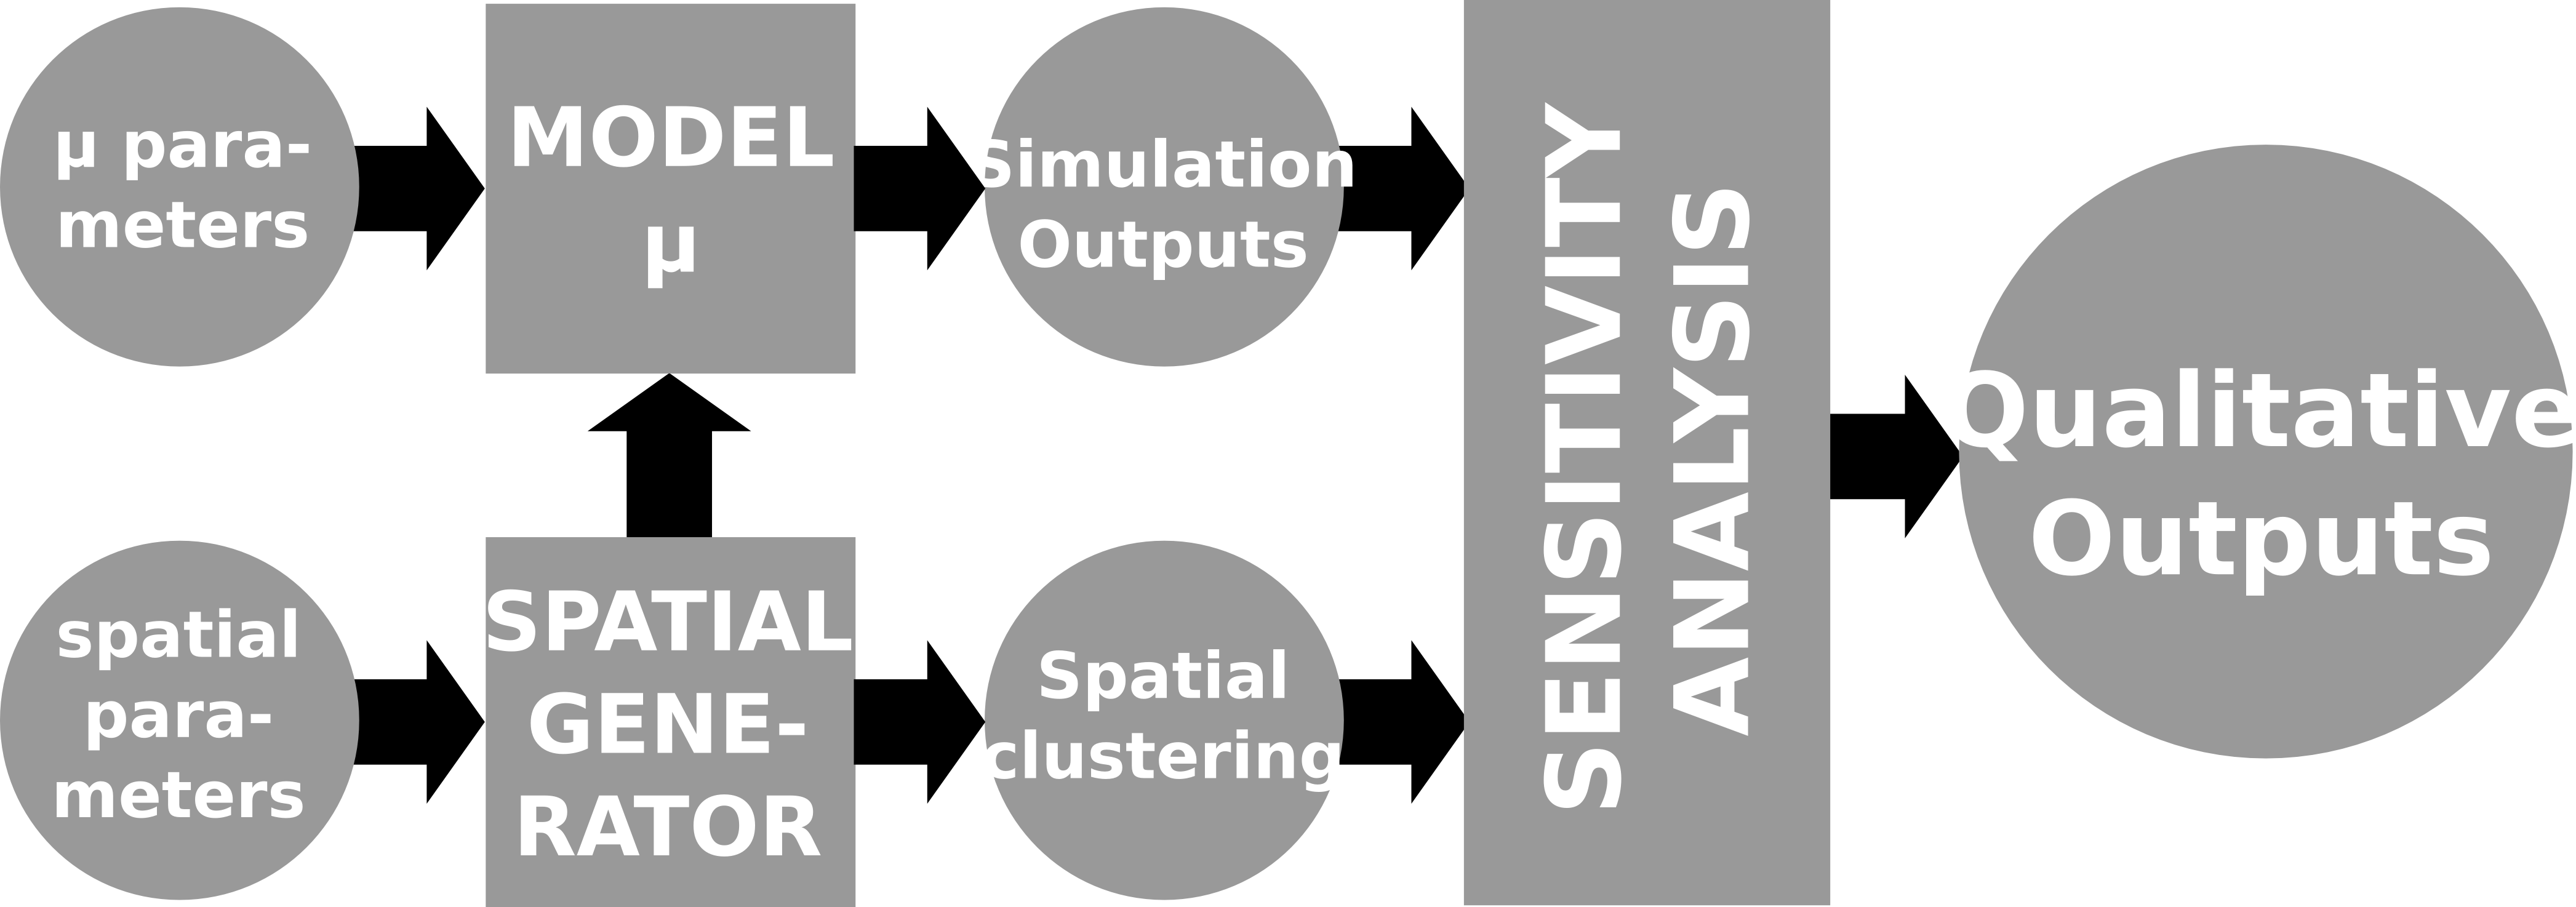
\includegraphics{figures/SchemaMeta_1.png}
} \caption{\textbf{General workflow.}} \label{fig:method}
\end{center}
\end{figure*} %
%%%%%%%%%%%%%%%%%%%%%%


In order to test the influence of initial spatial conditions on model outputs, we use a systematic method to compare \emph{phase diagrams}. \added{Following} \citet{Gauvinetal2009}, we define a phase diagram as the vector of \added{final aggregated} model outputs considered as a function of model parameters. We have as many phase diagrams than we have spatial grids, which makes a qualitative visual comparison not realistic (with around 50 different spatial configurations for each model experiment). A solution is to use systematic quantitative procedures to compare them.
Technically, because of stochasticity, we represent the output of the model for a given combination of parameter values $\vec{P}$ as the median of the final values of an output indicator $O$ obtained for the replications of the model initialized with $\vec{P}$.\\

To our knowledge there exist no single well established method to compare phase diagrams in the agent-based modelling and geosimulation literature. We introduce a measure of the relative distance $d_r$ between two phase diagrams $\mu_{\vec{\alpha}_1}$ and $\mu_{\vec{\alpha}_2}$. Phase diagrams are denoted by a common function $\mu$ indexed by what we call \emph{meta-parameters} $\vec{\alpha}$, that capture the spatial configuration \footnote{in practice these can be parameters of an upstream model to generate the configuration, or a description of the configuration itself}. The $d_r$ measure is taken as the share of between-diagrams variability relative to their internal variability, given formally in the case of a one-dimensional phase diagram by

%\comment[FL]{je ne comprends pas ce choix : pourquoi faut il considérer que des classes ayant une forte cohérence interne seraient plus éloignées? ou alors la question ne se pose pas en ces termes... Par ailleurs est ce que la formule est bien homogène du point de vue des dimensions? En tous cas je pense qu'on peut se passer de la formule à ce stade, éventuellement à mettre dans l'affichage des résultats si on en a besoin.}[(JR) pour l'homogénéité oui justement on prend $d^2$ car c'est les variances, on obtient une mesure sans unité ; ok pour omettre la formule ; pour l'interprétation, on regarde la distance relative, pour des classes à une certaine distance, si elles sont concentrées, cette distance sera plus sigificative que si elles ont une grande variabilité et peuvent se recouper ; par exemple si elles ont mêmes variance $\sigma^2$, alors si $d \simeq \sqrt{2} \sigma$ alors les nuages de points vont en gros se recouper sur leur moitié (cas gaussien idéal), tandis que si $d\gg \sigma$, le max d'un diagramme sera très loin du min de l'autre - on compare à la fois la distance relative et la distance de forme.]

%Several potential methods from other fields such as environmental science could be used, but we keep it simple and such methodological considerations are furthermore auxiliary to the main purpose of this paper. We propose therefore an intuitive measure corresponding to the share of between-diagrams variability relative to their internal variability. More formally, the distance is given by

\begin{equation}\label{eq:phase-distance}
d_r\left(\mu_{\vec{\alpha}_1},\mu_{\vec{\alpha}_2}\right) = 2 \cdot \frac{d(\mu_{\vec{\alpha}_1},\mu_{\vec{\alpha}_2})^2}{Var\left[\mu_{\vec{\alpha}_1}\right] + Var\left[\mu_{\vec{\alpha}_2}\right]}
\end{equation}

where $\mu_{\vec{\alpha}_i}$ are the phase diagrams at given meta-parameters $\vec{\alpha}_i$. $d$ is a functional distance that we take simply as Euclidian distance. The \replaced{internal variabilities}{variance} are estimated \added{as the variance} within each phase diagram $f_{\vec{\alpha_i}}$. For a multi-dimensional phase diagram, we sum these relative distances over the components. 

The last methodological point which we need to emphasize is the relation between the present workflow and model exploration workflows in general. The ideas of multi-modeling and extensive model exploration are nothing from new as ~\cite{openshaw1983data} already advocated for ``model-crunching'', but their effective use only begins to emerge thanks to the development of new methods and tools together with an explosion of computation capabilities. The model exploration platform OpenMOLE~\citep{reuillon2013openmole} allows to embed any model as a blackbox, to write modulable exploration workflow using advanced methodologies such as genetic algorithms and to distribute transparently the computation on large scale computation infrastructures such as clusters or computation grids. In our case, this tool is a powerful way to embed both the sensitivity analysis and the meta-sensitivity analysis, and to allow the coupling of any spatial generator with any model in a straightforward way as long as the model can take its spatial configuration as an input or from an input file. In this paper, we use the OpenMOLE platform for the spatial environment and the model coupling, placing ourselves in the  framework of multi-modelling \citep{cottineau2015modular}.


%%%%%%%%%%%%%%%%%%%%%%
\subsection{Spatial generator of density grids}

The spatial generator applies an urban morphogenesis model \citep{Batty2007} which has been generalised, explored and calibrated by~\citet{2017arXiv170806743R}. An open implementation and a characterisation of the urban forms which the model can produce \deleted{are provided, which} allow us to integrate it easily in our workflow. \deleted{In a nutshell, g}Grids are generated through an iterative process which, starting from a void grid, adds a quantity $N$ (population) at each time step $t$, allocating it through preferential attachment on population density, characterised by its strength of attraction $\alpha$. More precisely, each added unit has a probability equal to $P_i^{\alpha}/\sum_k P_k^{\alpha}$ to be added to \added{a} patch $i$ with population $P_i$, all $N$ units being added independently and in parallel. At the end of each time step, this growth process is smoothed $n_d$ times using a diffusion process of strength $\beta$: each patch transmits an equal share of $\beta\cdot P_i$ to its Moore neighborhood (8 surrounding patches). To avoid border effects such as a reflexion on the border of the world, border patches diffuse to the outside. The procedure stops when a fixed number of steps $t_f$ is reached. The grid then has a population of $t_f \cdot N$ (the population lost due to diffusion process to the outside is reallocated through a normalization procedure at the end of the steps). Grids are thus generated from the combination of the values of these four meta-parameters $\alpha$, $\beta$, $n_d$ and $N$, in addition to the random seed. To ease our exploration, only the distribution of density is allowed to vary rather than the size of the grid, which we fix to a 50x50 square environment. We furthermore fix the total population at $t_f\cdot N = 100,000$, and determine therein the number of steps needed at a given $N$. Typical value ranges for the  parameters will be taken as, following \citet{2017arXiv170806743R}, $\alpha\in\left[0.5,4.0\right]$, $\beta \in\left[0,0.3\right] $, $N\in \left[100,10000\right]$, $n_d\in\left[1,4\right]$. We illustrate in Fig.\ref{fig:spatialGen} the variety of spatial configurations that can be generated.

%%%%%%%%%%%%%%%%%%%%%%
\begin{figure*}[htbp] \begin{center} 
\resizebox{0.9\textwidth}{!}{ 
	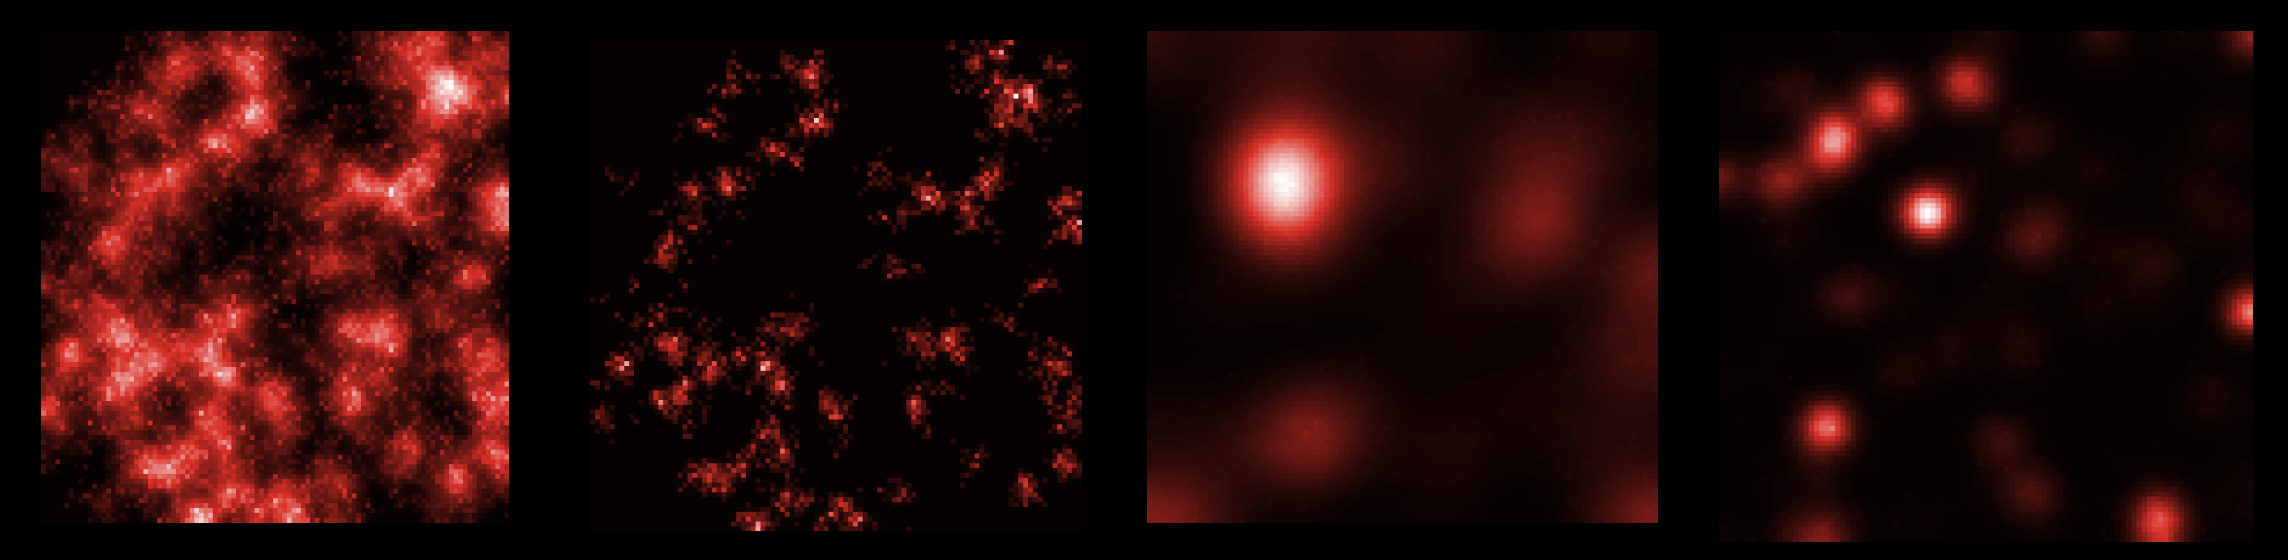
\includegraphics{figures/spatialGen.png}
} \caption{Four examples of grids produced by the spatial generator. The lighter the red, the denser the area. Changing the growth rate $N$ allows to have more or less chaotic shapes (two first compared to the two last grids for example) corresponding to different levels of convergence of the model, whereas local radius can be tuned with the interplay of aggregation strength $\alpha$ and diffusion strength $\beta$.} \label{fig:spatialGen} \end{center} \end{figure*} %
%%%%%%%%%%%%%%%%%%%%%%


%%%%%%%%%%%%%%%%%%%%%%
%\subsection{Including a (typical) variety of initial conditions in the sensitivity analysis}

In order to generate density grids which correspond to empirical density distributions, we select among the generated grids using an objective function which matches the point cloud of 110 metropolitan areas in Europe described by four dimensions of spatial structure: their concentration index, hierarchy index, centrality index and continuity index (cf. \cite{LeNechet2015}). We sample the meta-parameter space using a Latin Hypercube Sampling, which is a convenient technique to have a point cloud with high discrepancy. We sample 2000 points in the 4-dimensional space of parameters {$\alpha$, $\beta$, $n_d$, $N$}. It yields a subset of 170 interesting grids matching empirical densities, which constituted our set of different initial spatial conditions. These are further clustered into three classes of morphology (figure \ref{fig:densityTypes}): compact (e.g. Vienna), polycentric (Liege) and discontinuous (Augsburg). This clustering allows to evaluate the non-trivial effects of a meaningful urban form on simulation results. We select 15 grids of each type to work with in the computation of sensitivity analysis of an intra-urban model \deleted{, obtaining a total of 45 spatial configurations to compare (as we will see, the significant number of model runs needed to establish each phase diagram imposes a computational limit on this number of configurations)}(cf. section \ref{sec:qualResults}).

%%%%%%%%%%%%%%%%%%%%%%
\begin{figure*}[htbp] \begin{center} 
\resizebox{0.9\textwidth}{!}{ 
	\includegraphics{figures/GridPresentation.png}
} \caption{Correspondence between European urban density structures and grids produced with the spatial generator.} 
\label{fig:densityTypes} \end{center} \end{figure*} %
%%%%%%%%%%%%%%%%%%%%%%

In the following section, we briefly recall the main components of the two ``classical'' agent-based simulation models used to test how spatial density variations may impact simulation models behaviour and results, and how general the method is.

\subsection{Case study models}


Schelling's model consists in an abstract urban housing market where agents of different attributes (for example: red or green) sense their environment, evaluate their satisfaction in terms of neighbourhood composition (how many reds and greens?), and relocate if unsatisfied. It has been shown by \cite{Schelling1969} that even tolerant agents tend to produce segregated patterns because of the complexity of their local interactions \added{and the snowball effect of individual moves on the global distribution of agents in the city}. The main parameters of this model are the tolerance level (\added{maximum} \% of agents different to {\it ego} \added{accepted in the neighbourhood}), the scope of sensing, the minority split and the percentage of vacant spaces in the housing market. In addition, we are interested in testing the impact of the \added{initial} spatial distribution of housing capacity in this project, using the generated grids. The outcome of the model is measured \replaced{by a combination of three segregation indices:}{as a phase diagram of segregation level, described by the combination of several indicators:} Dissimilarity, Moran's Index, Entropy~\citep{brown2006spatial}. We translated the Netlogo implementation of Schelling into Scala for this project.

Sugarscape is a model of resource extraction which simulates the unequal distribution of wealth within a heterogenous population \citep{EpsteinAxtell1996}. Although it {\it "is designed to study the interaction of many plausible social mechanisms"} \citep[p.125]{Axtelletal1996}, we refer in this paper to the first (and simplest) version of the model, where {\it "processes allow its agents to look for, move to, and eat a resource ("sugar") which grows on its \replaced{[...]}{toroidal} array of cells"}. Agents of different vision scopes and different metabolisms harvest a self-regenerating resource available heterogeneously in the initial landscape, they settle and collect this resource, which leads some of them to survive and others to perish. The main parameters of this model are the number of agents, their minimal and maximal resource levels. In addition, we are interested in testing the impact of the spatial distribution of the resource, using the generated grids. We extend the implementation with agents wealth distribution of~\citet{li2009netlogo}. The outcome of the model is measured \replaced{by a Gini}{ as a phase diagram of an} index of inequality for resource distribution.\deleted{(Gini index)}. 


\subsection{Experiment design}
For Sugarscape, we explore three dimensions of the parameter space: the total population of agents $P\in \left[10;510\right]$, the minimal initial agent resource $s_{-}\in \left[10;100\right]$ and the maximal initial agent resource $s_{+}\in \left[110;200\right]$. Each parameter is binned into 10 values, giving 1000 parameter points. We run 50 repetitions for each configuration, which yields reasonable convergence properties. The initial spatial configuration varies across 50 different grids, generated by sampling meta-parameters for the generator in a LHS. We did not use the clustered grids to test the flexibility of our framework, which is demonstrated in this case by a direct sequential coupling of the generator and the model. Indeed, because the density distribution refers to the distribution of resource rather than to the representation of a city structure, we do not need the typology of urban density in this experiment. The full experiment thus equates to 2,500,000 simulations (1000 parameter combinations x 50 density grids x 50 replications). 

For Schelling's model, we also explore three dimensions of the parameter space of the model: the minimum proportion of similar agents required in the neighbourhood for the agent to be satisfied (or intolerance level) $S\in \left[0;1\right]$, the initial split of population, derived from the proportion of green population, $G\in \left[0;1\right]$ and the vacancy rate of the city $V\in \left[0;1\right]$. We sample 1000 parameter values using a Sobol sampling and run 100 repetitions for each configuration. We first try the same experiment design (50 density grids generated on the fly), then look at clustered grids representing urban densities. We choose 45 different grids among the ones which are most representative of the three types of urban morphology: 15 compact grids \deleted{(like Vienna, cf figure 3)}, 15 polycentric grids \deleted{(like Liege)} and 15 discontinuous grids \deleted{(like Augsburg)}. The last experiment thus equates to 4,500,000 simulations (1000 parameter combinations x 45 density grids x 100 replications). We use OpenMOLE to distribute the computation, and apply segregation measures to characterise the results.



We choose different experiment designs, both for meta-parameters and for the phase diagram, to demonstrate the robustness of the method to technical choices. In principle, our workflow applies with \replaced{to}{any} manner to generate a spatial configuration (even taking real configurations) and any manner to establish phase diagrams.




%%%%%%%%%%%%%%%%%%%%%%
\section{Results}
%%%%%%%%%%%%%%%%%%%%%%

%\comment[FL]{il faudrait peut être davantage renforcer l'analyse a propos de figure 1 de si c'est plutôt les mu parameters ou les spatial parameters qui ont une grosse influence sur les résultats.}[(JR) assez explicite pour sugarscape, j'ai rajouté un peu tout de même.]

\subsection{Quantitative variation across grids}

We measure the distance of the phase diagrams for all density grids with respect to the reference phase diagram computed on the default \replaced{initial spatial condition}{model} setup (a bi-centric symmetric\added{al non toroidal} configuration) using the \deleted{relative} measure defined in equation~\ref{eq:phase-distance}. For each density grid, we \deleted{then} obtain the average squared distance between corresponding points of the phase diagrams, i.e. the median value of the final output measure, such as segregation or inequality, for a given value of parameters \added{in the two setups (isotropic and generated)}. This average squared distance for each point is then related to the average variance of each of the phase diagram (the reference one and the one for the grid under inquiry). Therefore, values greater than 1 will mean that inter-diagram variability is more important than intra-diagram variability.

\paragraph{Sugarscape} 


% summary stats
%   Min. 1st Qu.  Median    Mean 3rd Qu.    Max. 
% 0.08909 0.19790 1.52200 1.29600 2.16400 2.98100 

We obtain a very strong sensitivity to initial spatial conditions for the Sugarscape model. Indeed, the relative distance between the phase diagrams of different density grids and the phase diagram of the reference case ranges from 0.09 to 2.98 with a median of 1.52 and an average value of 1.30. The mean distance above 1 means that, on average, the model is more sensitive to meta-parameters of grid generation than to its own parameters (population and sugar endowment) in the reference model. Moreover, the maximum distance of 2.98 means that the variation due to the change of grid can be up to three times bigger than the variation due to the model parameters. We plot in Fig.~\ref{fig:sugarscape-distance-meta} the distribution of these distances in \replaced{the meta-parameter}{a morphological} space. Each point represent one of the 50 different density grids used to initialise the distribution of sugar in the model. The points are projected with respect to the meta-parameters used to generate the grid, and coloured according to the relative distance of the phase diagram of the simulations using this grid to the phase diagram of the reference case. Therefore, the figure ~\ref{fig:sugarscape-distance-meta} shows that the grids generated with a high $\alpha$ (i.e. with a small number of very high density cells) produce simulation results \replaced{that vary more between the reference case and the generated grid with the sa,e values of parameters than within the reference case because}{more different compared to the reference case than within this reference case because} of parameter variations. This pattern is emphasized when grids are generated with a high $\alpha$ and a high $\beta$ (i.e. with low gradient of density decrease around the kernels of high density). These grids have the highest relative distance to the reference case. On the contrary, with grids closer to the uniform pattern of the reference case (bottom left of the graph), the model parameters are more important in determining the \replaced{final inequality levels than the initial spatial distribution of sugar}{simulation results}. 


%%%%%%%%%%%%%
\begin{figure}
\centering
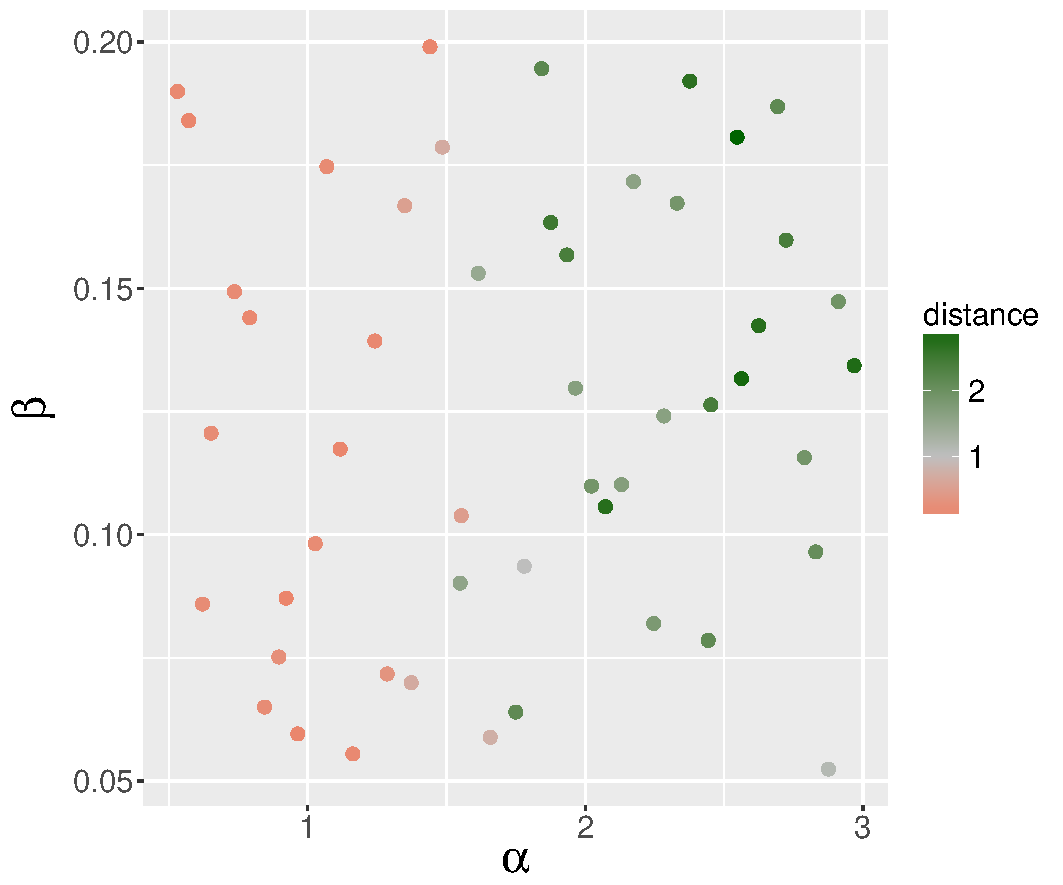
\includegraphics[width=0.8\textwidth]{figures/relativedistance_metaparams}\\
%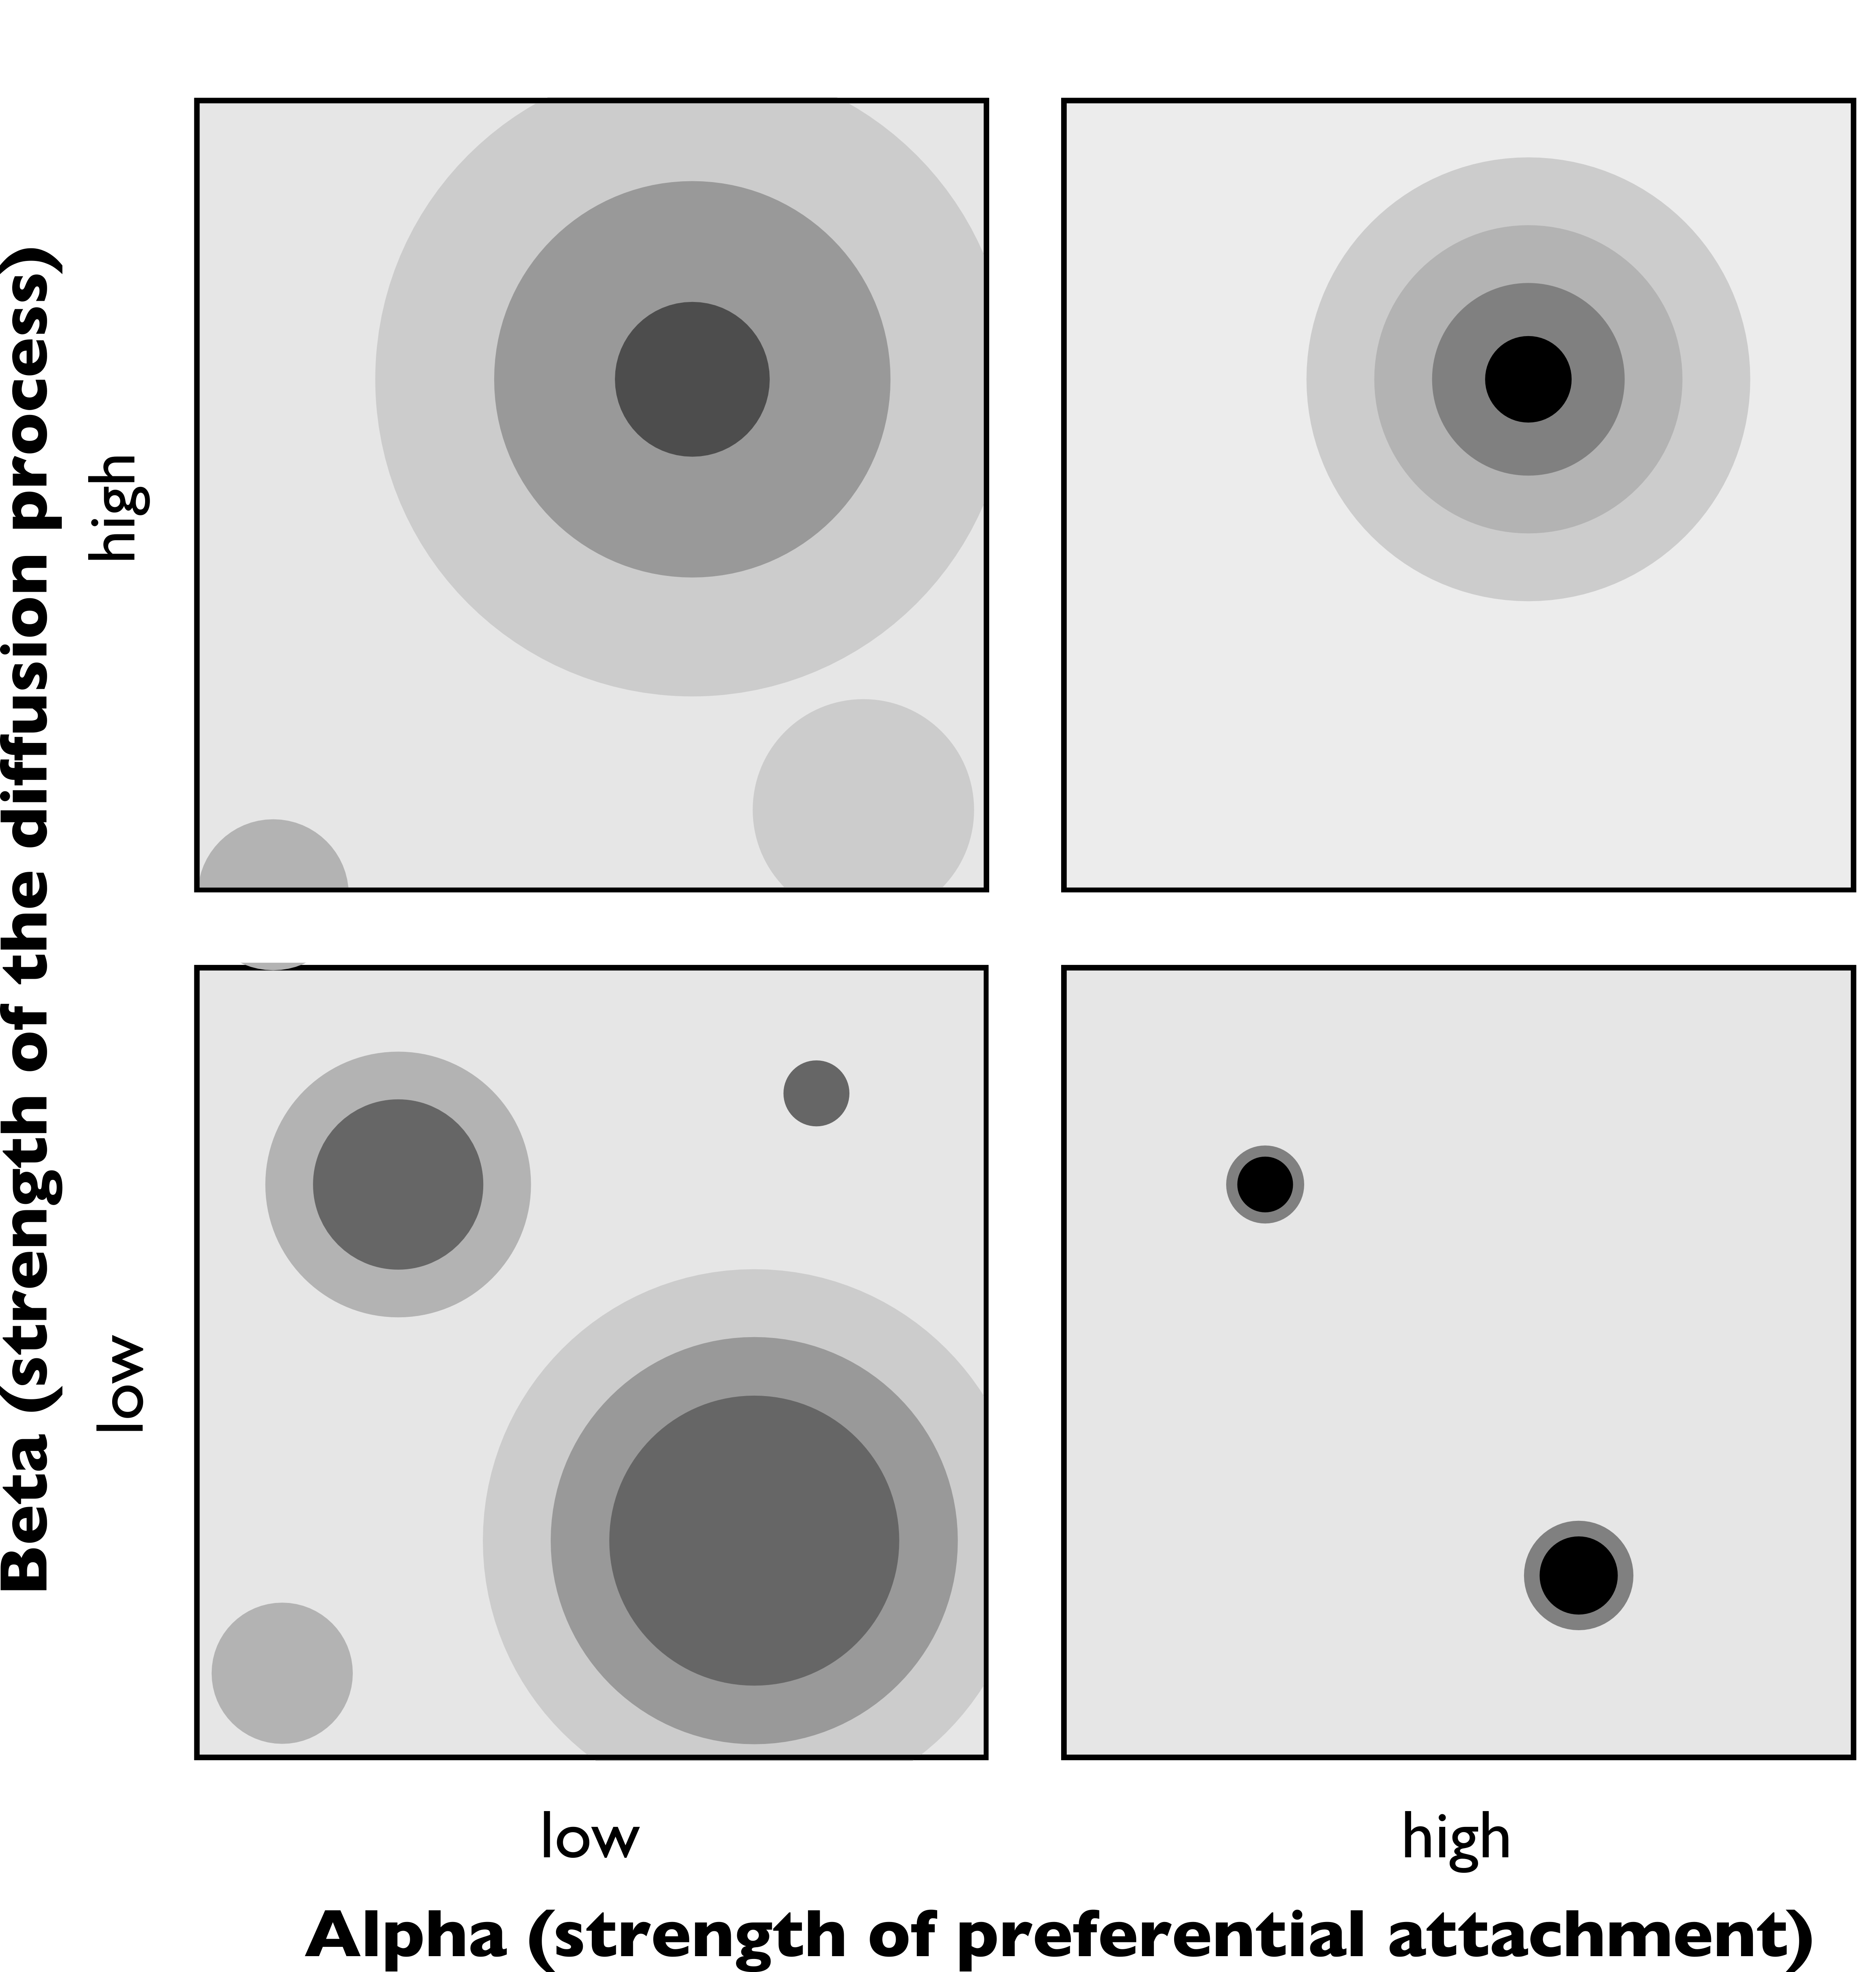
\includegraphics[width=0.4\textwidth]{figures/alpha_beta_schemas}(Bottom) Corresponding stylised density grids\\\comment[JR]{je sais pas si c'est une bonne idee de mettre les grilles stylisees comme ca parce que ca donne une fausse idee des sorties du modele de generation}}
\caption{\textbf{Relative distances of phase diagrams by initial spatial grids described by the meta-parameters of their generator.} Relative distance as a function of meta-parameters $\alpha$ (strength of preferential attachment) and $\beta$ (strength of diffusion process).}
\label{fig:sugarscape-distance-meta}
\end{figure}
%%%%%%%%%%%%%

Another way of quantifying the density grids, instead of looking at the meta-parameters of their generator, is to look at the resulting indicators of urban form, such as Moran index, average distance, rank-size slope and entropy (see~\cite{LeNechet2015} for precise definition and context). This 4-dimensional space defined a morphological space. For the purpose of interpretability and visualisation, we reduce this space to a bi-dimensional space with a principal component analysis. The first two components represent 92\% of cumulated variance. The first component defines a ``level of sprawl'' and of scattering, whereas the second one represents the level aggregation.\footnote{We have $PC1 = 0.76\cdot distance + 0.60\cdot entropy + 0.03\cdot moran + 0.24\cdot slope$ and $PC2 = -0.26\cdot distance + 0.18\cdot entropy + 0.91\cdot moran + 0.26\cdot slope$.} We find that grids producing the highest deviations are the ones with a low level of sprawl and a high aggregation (top left of figure \ref{fig:sugarscape-distance-pca}). It is confirmed by the behaviour as a function of meta-parameters, as high values of $\alpha$ also yield high distance. In terms of model processes, it shows that congestion mechanisms in the gathering of the resource induces fast increases of inequality. To put these results in perspective of our workflow given in Fig.~\ref{fig:method}, we have a sensitivity to spatial parameters on average greater than the sensitivity to model parameters.

% pca of morphological space
% "","PC1","PC2","PC3","PC4"
%"distance",0.762358566609464,-0.260991693298744,0.200656405132039,0.557162237616392
%"entropy",0.601306167355116,0.181706245959277,0.0958379422351422,-0.772158547261002
%"moran",0.0311129390452153,0.912155429075071,0.30114271129527,0.276256268103684
%"slope",0.237217819823539,0.258531718397015,-0.927289147645628,0.130475642169329

%%%%%%%%%%%%%
\begin{figure}
\centering
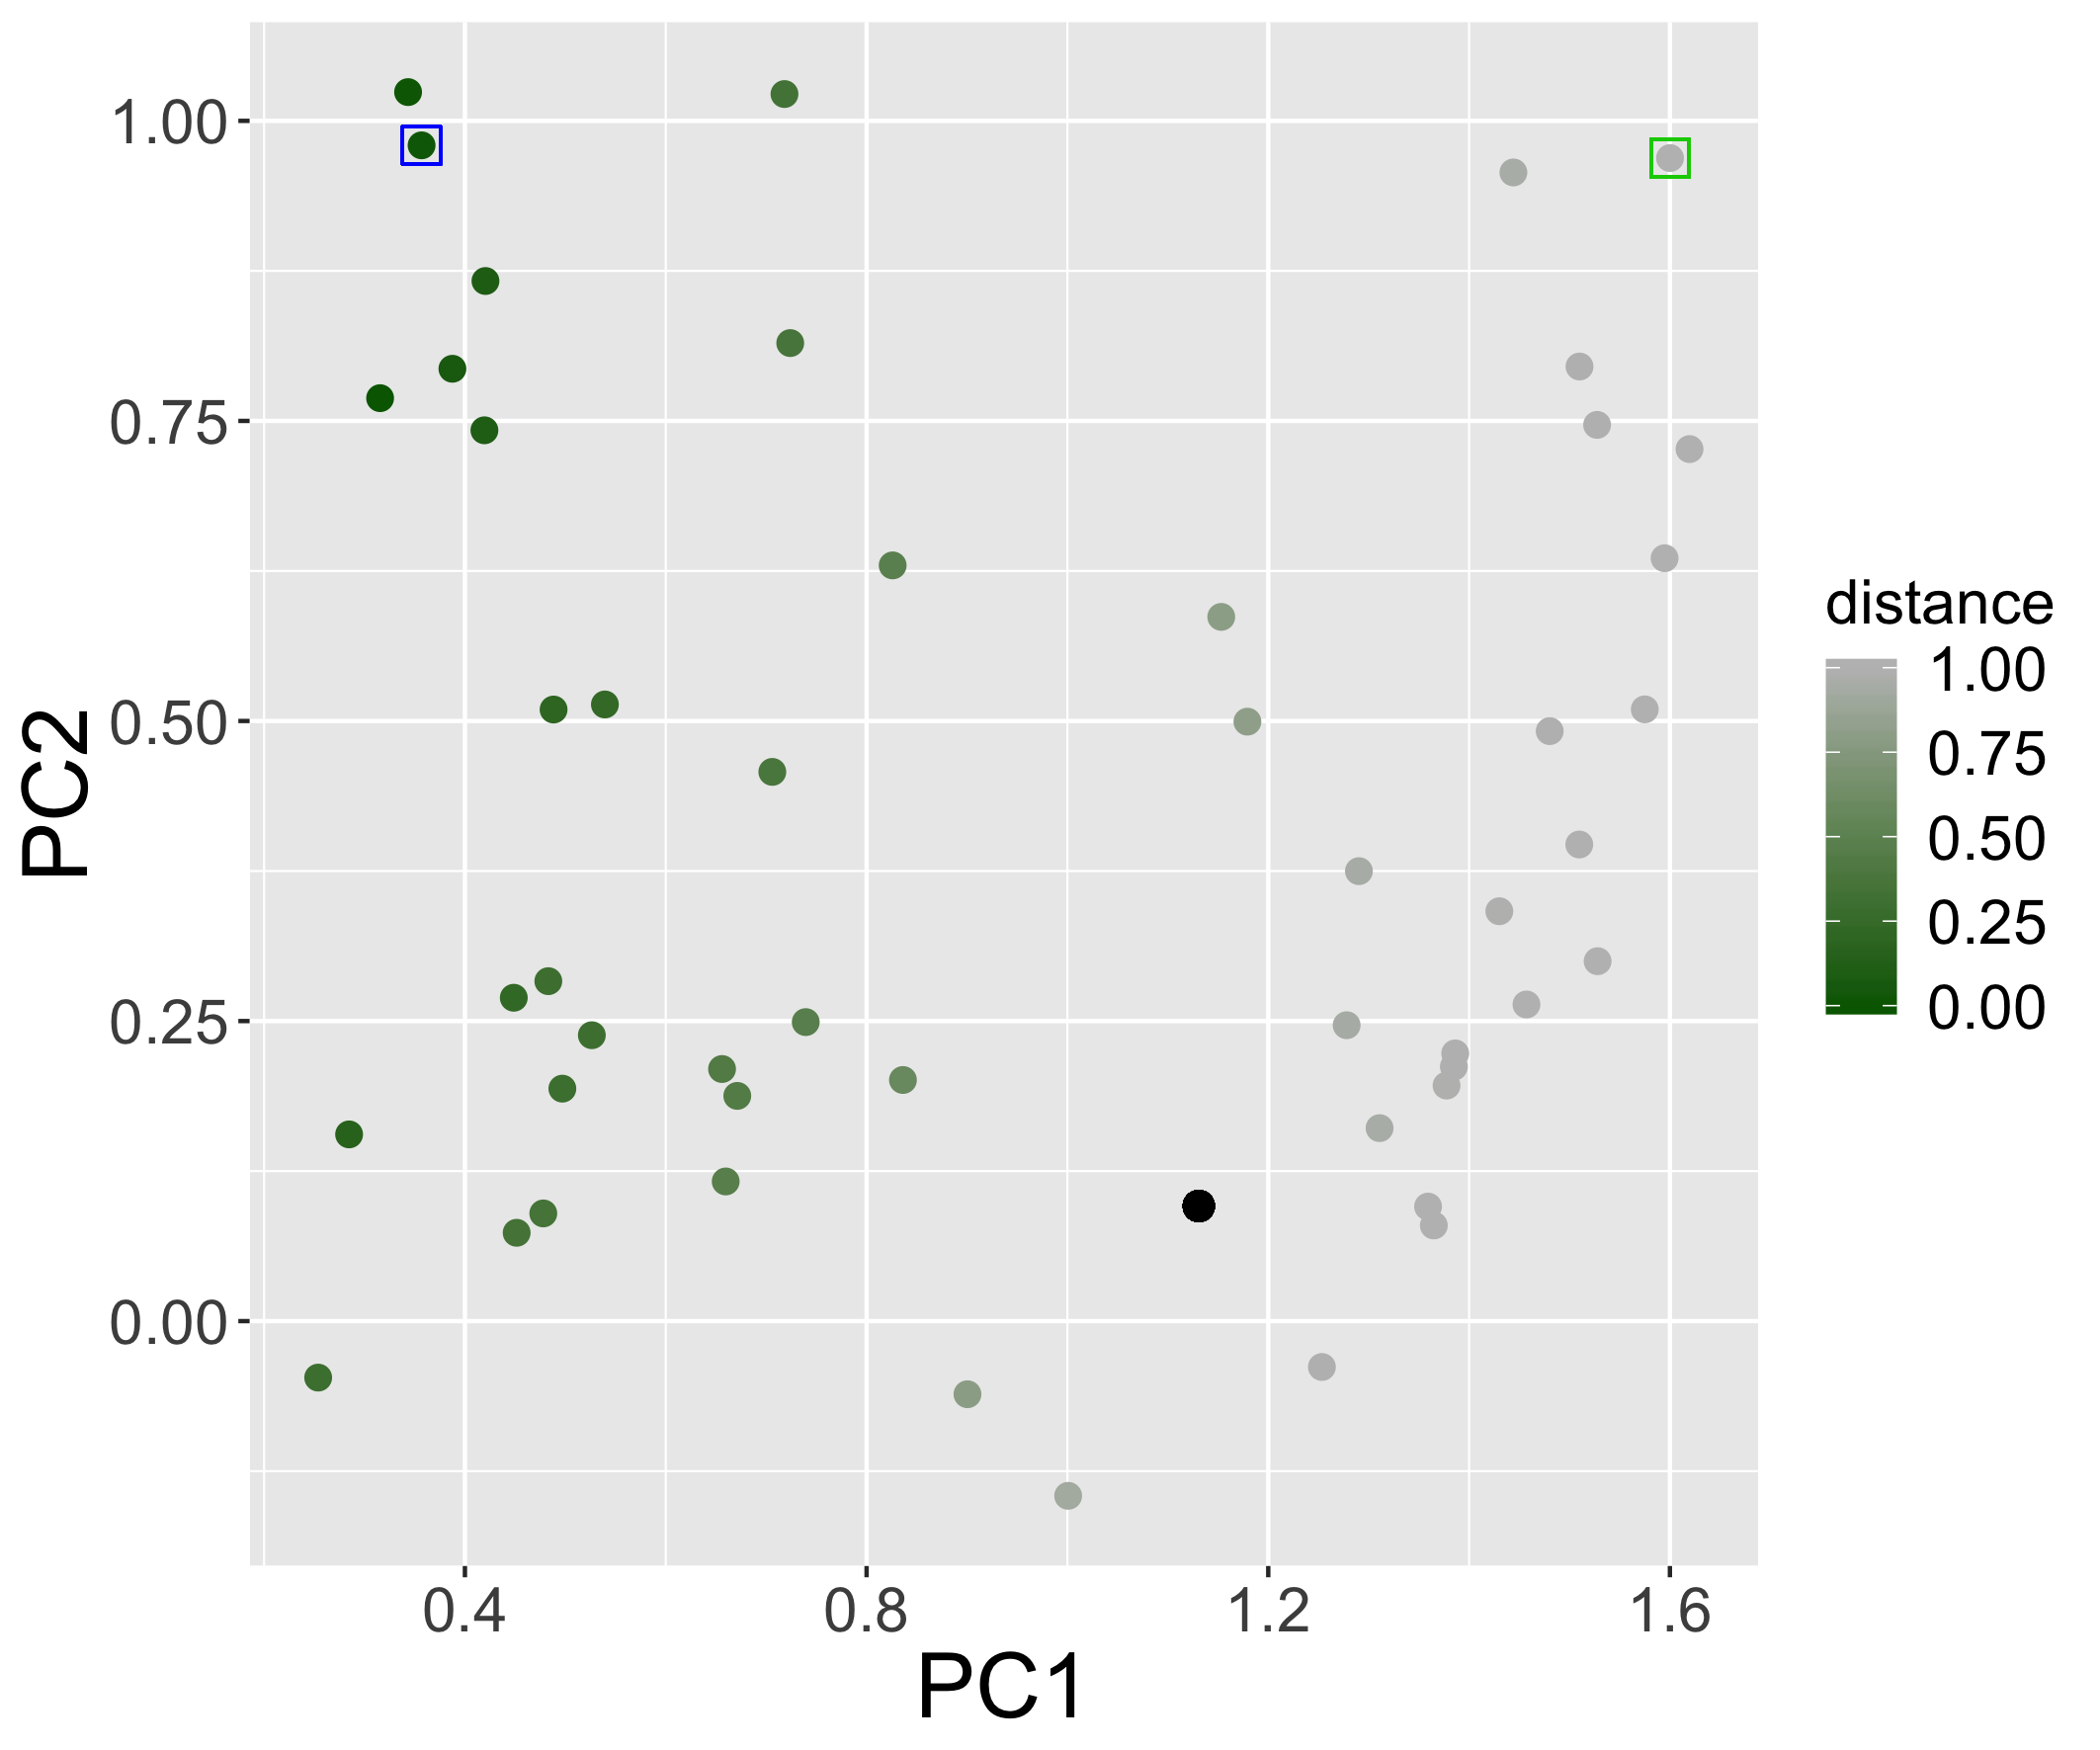
\includegraphics[width=0.8\textwidth]{figures/relativedistance_morphspace}
\caption{\textbf{Relative distances of phase diagrams to the reference across grids.} Relative distance as a function of two first principal components of the morphological space (see text). Black point correspond to the reference spatial configuration. Green frame and blue frame give respectively the first and second particular phase diagrams shown in Fig.~\ref{fig:sugarscape-phasediagrams}.}
\label{fig:sugarscape-distance-pca}
\end{figure}
%%%%%%%%%%%%%

\paragraph{Schelling} 
Within a standard Schelling model (i.e. initialised with a uniform density grid), \citet{Gauvinetal2009} have built the phase diagram of segregation patterns depending on the combination of parameter values. For high levels of tolerance ($S < 0.25$), there is no segregation. For high values of vacancies ($V > 0.65$) and low values of tolerance ($S > 0.5$), these is a diluted segregation state where homogeneous communities are separated from other by large empty buffers. Finally, for low values of vacancies ($V < 0.2$) and low values of tolerance ($S > 0.7$), the model is frozen in a state where everyone is unhappy but no-one can express their intolerant behaviour due to the lack of free spaces. Between these extreme cases, the model gives rise to segregated states where homogeneous communities adjoin one another. The objective of this quantitative experiment is to evaluate to which extent this phase diagram is modified when different density grids are applied. We show in Fig.\ref{fig:schelling-distance-meta} (Supplementary Material) the values of the relative distance as a function of meta-parameters and in the reduced morphological space, in a way similar to the analyse done with Sugarscape\deleted{ before}. Variations are less considerable than for Sugarscape across phase diagrams, but values close to 1 show that several configurations are as \deleted{much} sensitive to \replaced{initial spatial conditions}{space} than to their parameters. We \deleted{will} focus in the following \replaced{on}{in} a qualitative characterisation of \added{these} variations.

\subsection{Qualitative variations}
\label{sec:qualResults}

\paragraph{Schelling} In this qualitative exploration of the effect of initial spatial conditions on the results of Schelling's model, we use the classification of grids into three morphological types (cf. figure \ref{fig:densityTypes}). In particular, we want \added{to} evaluate to which extent the typology summarises the spatial effects, and \deleted{so} if one type of urban form or \replaced{another}{the other} enhances\deleted{ or mutes} the segregation mechanism of the model, or interacts differently with the model parameters. This experiment \replaced{attempts at drawing}{aims at suggesting topical} conclusions on urban morphology, beyond the technical conclusions already obtained with respect to simulation sensitivity.





\begin{table*}[]
\centering
\begin{threeparttable}
\caption{\textbf{Regression of the segregation level of Schelling simulation with order parameters and type of city grid.}}
\label{tab:regressionSchelling}
%\begin{adjustwidth}{-1cm}{-1cm}
\begin{tabular}{|m{2.5cm}|ll|ll|ll|}
\hline
Simulation outcome by segregation index:    & \multicolumn{2}{c|}{\textbf{Dissimilarity}}   & \multicolumn{2}{c|}{\textbf{Entropy}} & \multicolumn{2}{c|}{\textbf{Moran's I}} \\ \hline
\textbf{Intercept}                          & -0.212 *** & -0.141 ***                       & -0.254 ***        & -0.208 ***        & -0.036 ***           & -0.061 ***               \\ \hline
\textbf{Similarity Wanted (S)}              & 1.212 ***  & 1.212 ***                        & 1.250 ***         & 1.250 ***         & 0.550 ***            & 0.550 ***                \\ 
\textbf{quadratic term ($S^2$)}               & -0.942 *** & -0.942 ***                       & -0.963 ***        & -0.963 ***        & -0.428 ***           & -0.438 ***               \\ 
\textbf{Vacancy Rate (V)}                   & 0.602 ***  & 0.602 ***                        & 0.453 ***         & 0.453 ***         & -0.027 ***           & -0.027 ***               \\ 
\textbf{Minority Index (\%Maj - \%Min)}     & 0.307å ***  & 0.307 ***                        & 0.130 ***         & 0.130 ***         & -0.067 ***           & -0.067 ***               \\ \hline
\textbf{Density Grid = Polycentric}         &            & 0.087 ***                        &                   & 0.052 ***         &                      & 0.001 ***                \\ 
\textbf{Density Grid = Discontinuous}       &            & 0.111 ***                        &                   & 0.068 ***         &                      & \textit{0.00}              \\
\textbf{Attraction meta-parameter $\alpha$} &            & -0.083 ***                       &                   & -0.053 ***        &                      & 0.014 ***                \\ 
\textbf{Diffusion meta-parameter $\beta$}   &            & 0.323 ***                        &                   & 0.218 ***         &                      & 0.017 ***           \\ \hline
\textbf{R2 (\%)}                            & 30.6       & 34.7                             & 24.1              & 25.6              & 23.9                 & 24.0                    \\ 
\textbf{\# of observations (sim. runs)}     & 2,106,000  & 2,106,000 						 & 2,106,000          & 2,106,000          & 2,106,000             & 2,106,000                \\ 
\textbf{AIC}                                & -70717.68   & -198748.2  						& 208213.8          & 166048.8          & -4385990             & -4387816                 \\ \hline
\end{tabular}
%\end{adjustwidth}
\begin{tablenotes}
 \item Moran's I applies to the minority population
 \item *** means that the estimate is significant at the 0.01 level.
\end{tablenotes}
  \end{threeparttable}
\end{table*}

In table \ref{tab:regressionSchelling}, we see that the type of density grid with which the model is initialised \replaced{correlates}{determines} to a certain extent \added{with} the level of segregation measured at the end of the simulation run. Indeed, compared to compact density patterns, polycentric grids produce more dissimilarity and entropy between the location of green and red agents. Discontinuous grids have the same effect, although attenuated. The results obtained with Moran's I are opposite, because this index measures spatial autocorrelation at the global level and that compact cities have higher levels of global autocorrelation by construction. However, linear models with and without \deleted{information about }the type of density distribution yield the same coefficients for Schelling's parameters $V$ and $S$, the only exception being the vacancy rate $V$ in the Moran's I model with grid types, which becomes non-significant. The similarity of the coefficient in both cases means that the effect of the model's parameters (and thus the mechanism by which agents of similar group cluster in space) is the same regardless of the distribution of density. The way polycentric and discontinuous density grid exhibit higher segregation is by allowing buffer zones of low density to surround pockets of homogeneity, which is impossible in a compact city, because everyone is at reach of everyone else. The buffering process confirms previous results obtained with network structures \citep{Banos2012} \added{and supports the conclusion that space acts here on top of mechanisms rather than in interaction with them}.

\paragraph{Sugarscape} We now check the sensitivity in terms of qualitative behavior of phase diagrams. We show the phase diagrams for two very opposite morphologies in terms of sprawling, but controlling for aggregation with the same $PC2$ value. These correspond to the green and blue frames in Fig.~\ref{fig:sugarscape-distance-pca}. In terms of grid shape, we observe that the difference between the two grids is mainly on average distance and entropy: in a nutshell, the first grid is much more dispersed and disorganised than the second. Although the behaviours are rather stable for varying $s_+$, the initial maximum endowment in sugar, which means that the poorest agents have a determinant role in trajectories, the two examples have not only a very distant baseline inequality (the ceiling of the first 0.35 is roughly the floor of the second 0.3), but their qualitative behavior is also radically opposite: the sprawled configuration gives inequalities decreasing as population decreases and decreasing as minimal wealth increases, whereas the concentrated one gives inequalities strongly increasing as population decreases and also decreasing with minimal weights but significantly only for large population values (fig. \ref{fig:sugarscape-phasediagrams}. In sprawled spaces, inequalities are thus fostered by a lack of minimal local resources, whereas population will drive inequality in concentrated spaces. The process is thus completely reversed depending on the grid chosen to run the model, which would have significant impacts if one tried to deduce policies from this model.
%This second example confirms thus the importance of sensitivity of simulation models to the initial spatial conditions.


% phase diagrams -> ok well different qualitatively
%          spAlpha spDiffsteps spDiffusion spGrowth spPopulation
% id=27 : 0.7913103    2.376837   0.1440293 157.4147 4852.746
% id=0 : 2.562398    3.753032   0.1316788 128.4632 4753.983
% maxSugar = 110


%%%%%%%%%%%%%
\begin{figure}
\centering
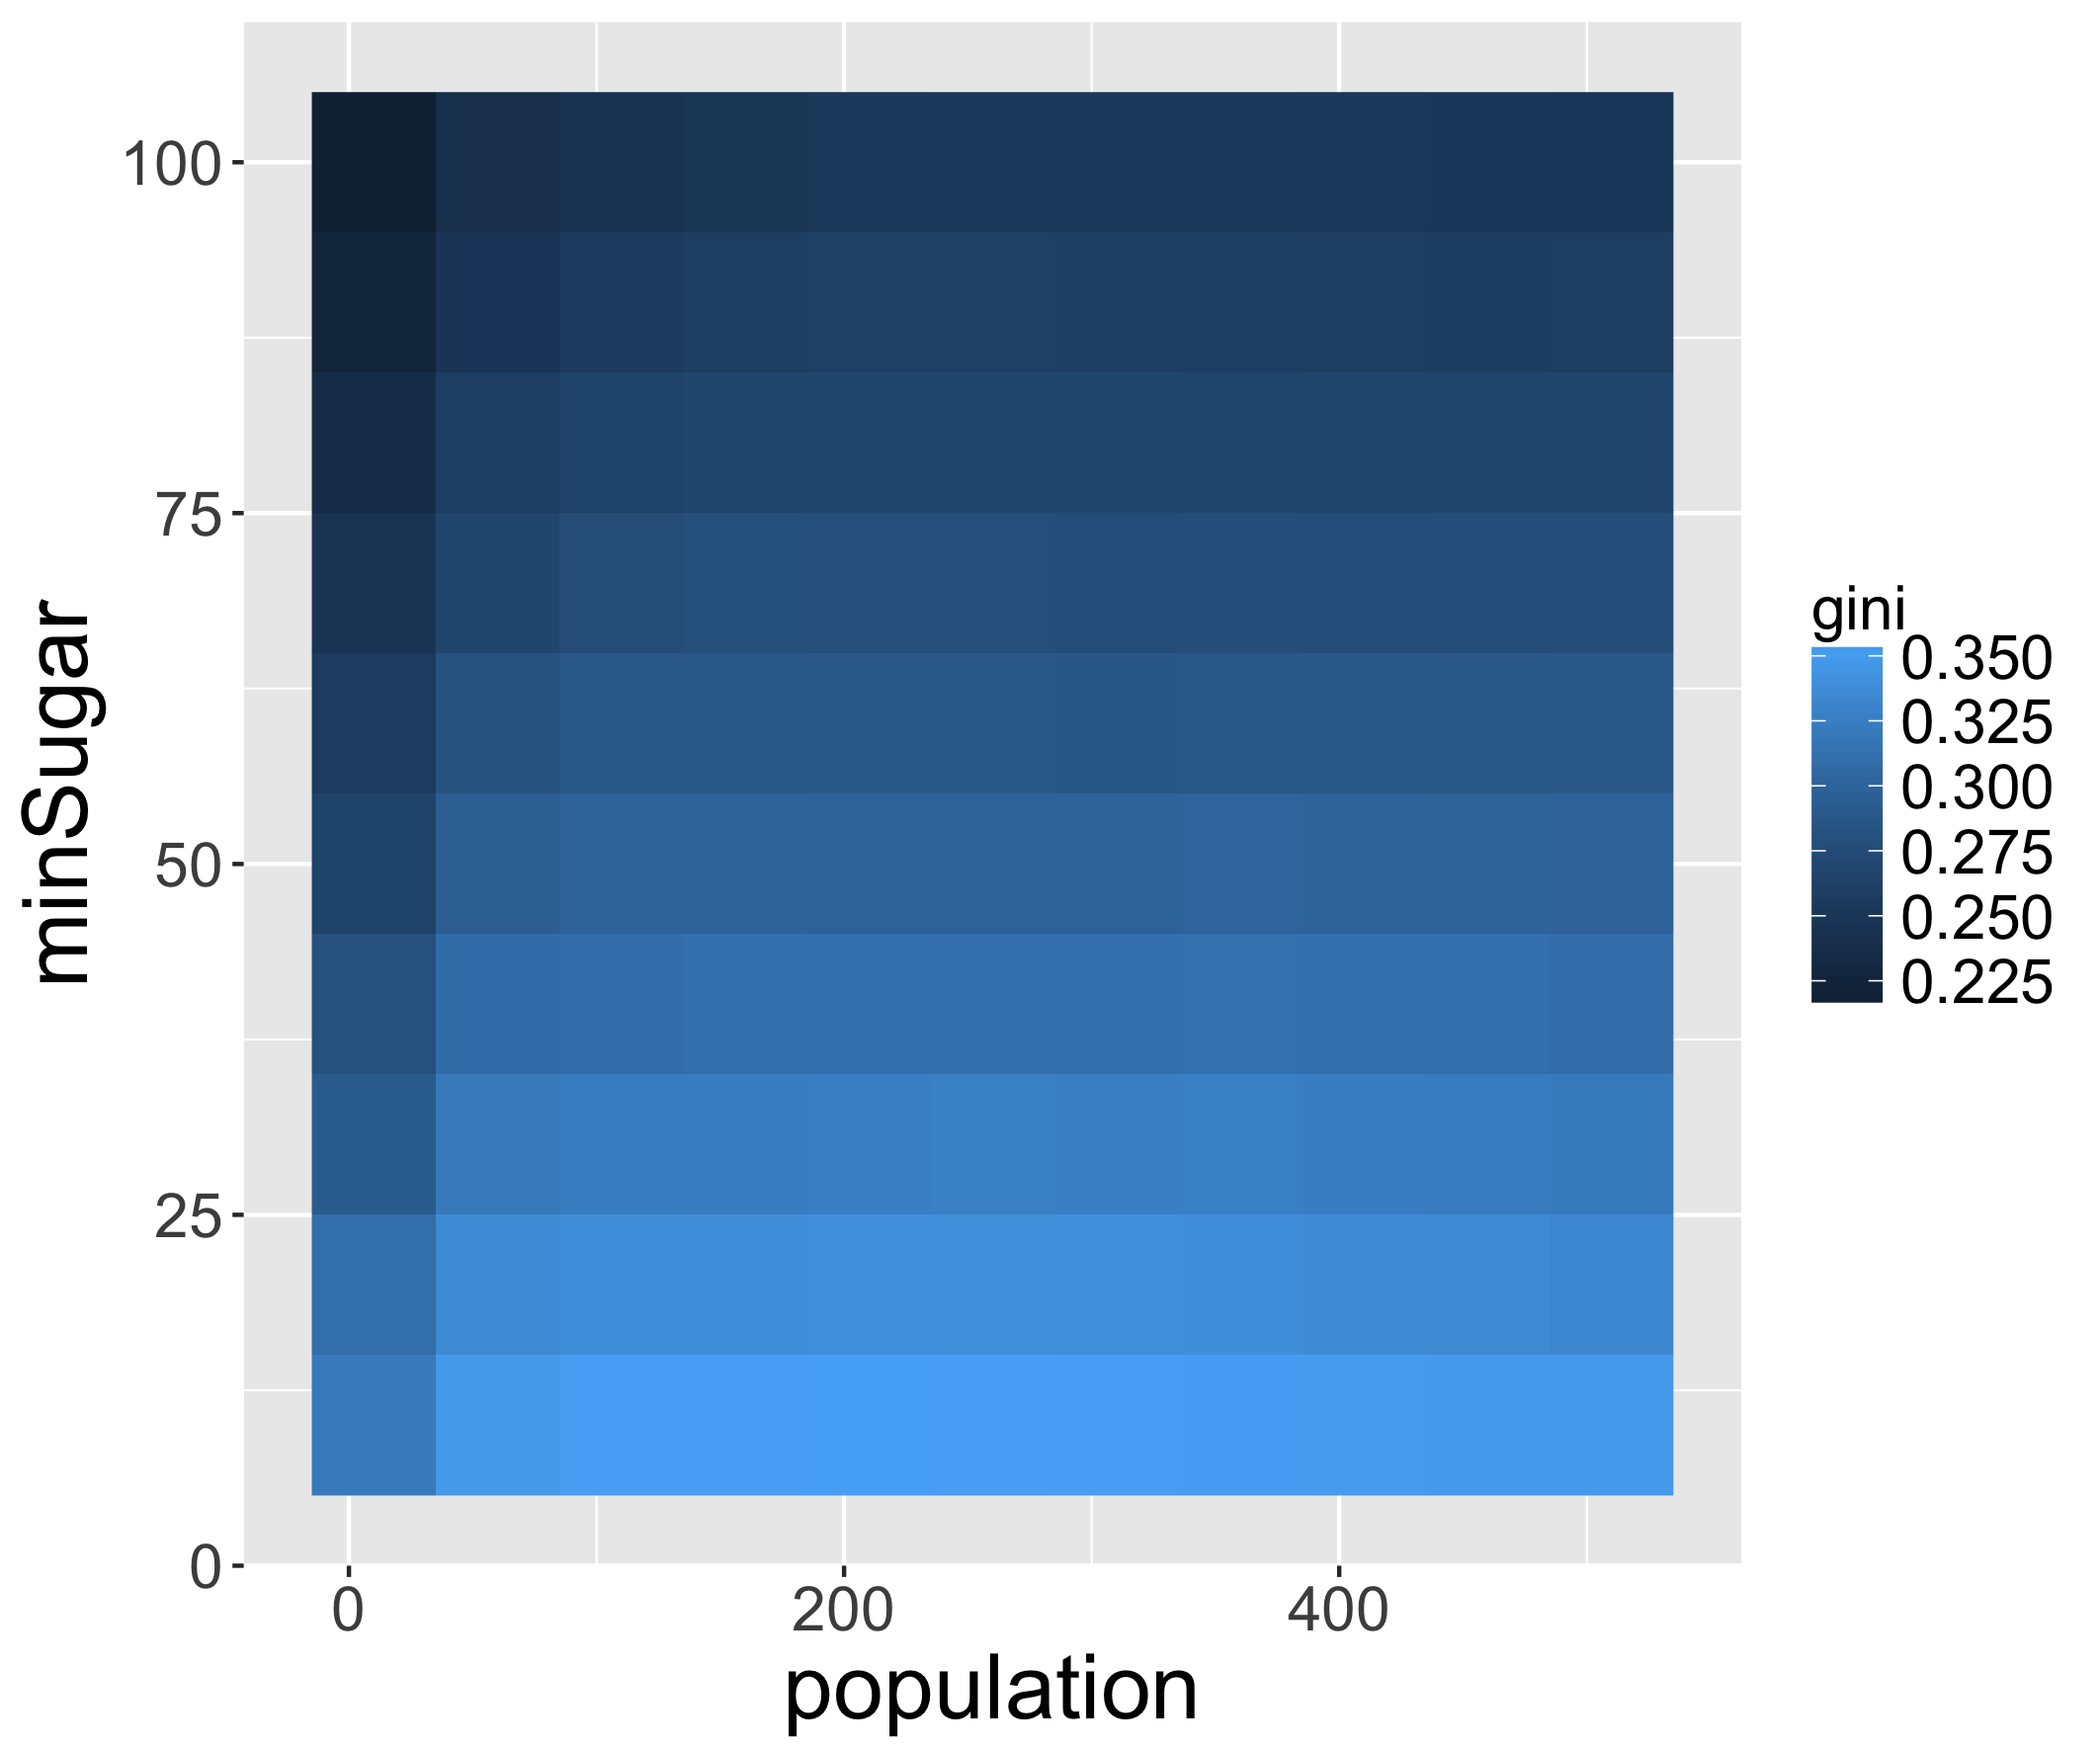
\includegraphics[width=0.48\textwidth]{figures/phasediagram_id27_maxSugar110}
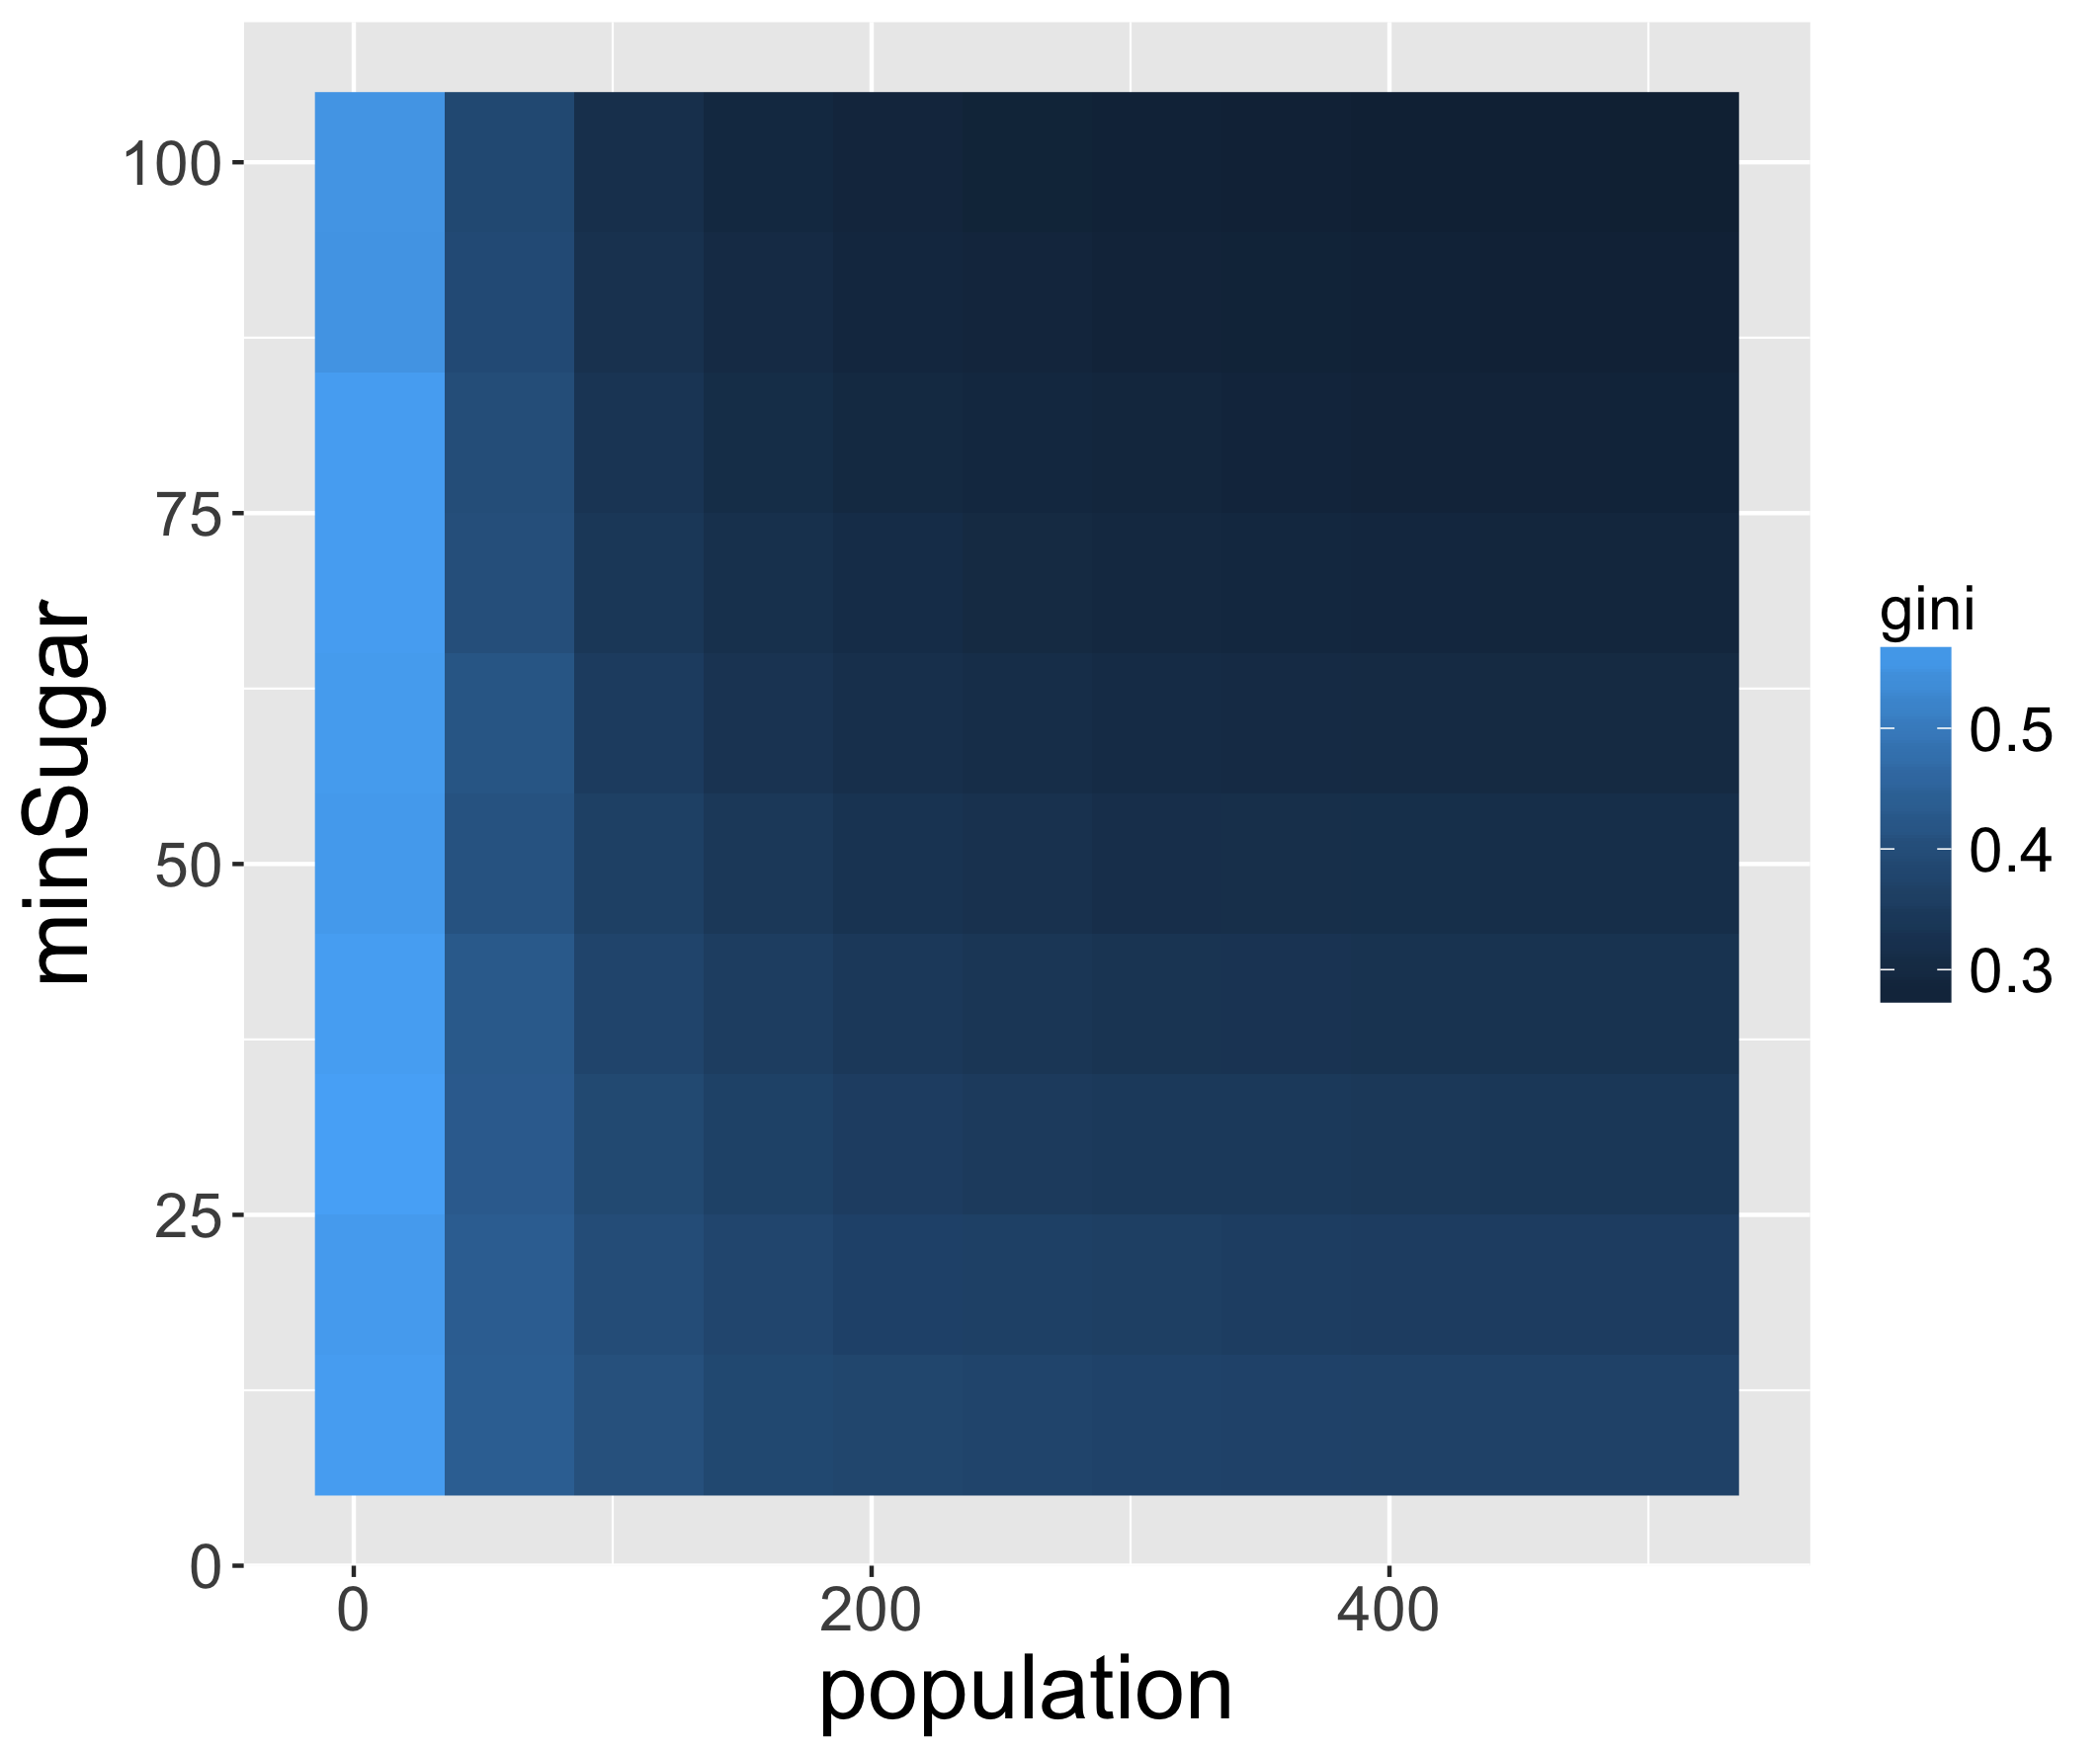
\includegraphics[width=0.48\textwidth]{figures/phasediagram_id0_maxSugar110}
\caption{\textbf{Examples of phase diagrams.} We show two dimensional phase diagrams on $(P,s_-)$, both at fixed $s_+ = 110$. (Left) Green frame, obtained with $\alpha = 0.79$, $n=2$, $\beta = 0.14$, $N=157$; (Right) Blue frame, obtained with $\alpha = 2.56$, $n=3$, $\beta = 0.13$, $N=128$.}
\label{fig:sugarscape-phasediagrams}
\end{figure}
%%%%%%%%%%%%%


%%%%%%%%%%%%%%%%%%%%%%
\section{Discussion}
%%%%%%%%%%%%%%%%%%%%%%

We consider that the method presented \added{in this paper} holds great potential for strengthening geographical models' exploration. However, two limits and two areas of opportunities have still not been tackled. 

\subsection{Limits}

\paragraph{Comparing phase diagrams} Comparing phase diagrams is as we saw not so straightforward, and further developments of our method imply testing alternative methods for this particular point. For example in the case of the Schelling model, an anisotropic spatial segregation index (giving the number of clusters found and in which region in the parameter spaces they are roughly situated) would differentiate strong \emph{meta phase transitions} (phase transitions in the space of meta parameters). The use of metrics comparing spatial distributions, such as the Earth Movers Distance which is used for example in Computer Vision to compare probability distributions~\citep{rubner2000earth}, or the comparison of aggregated transition matrices of the dynamic associated to the potential described by each distribution, would also be potential tools. Map comparison methods, popular in environmental sciences, provide numeral tools to compare two dimensional fields~\citep{visser2006map}. To compare a spatial field evolving in time, elaborated methods such as Empirical Orthogonal Functions that isolates temporal from spatial variations, would be applicable in our case by taking time as a parameter dimension, but these have been shown to perform similarly to direct visual inspection when averaged over a crowdsourcing~\citep{10.1371/journal.pone.0178165}. The investigation of diverse approaches to systematically quantify differences between phase diagrams is an important potential development of our method.


\paragraph{Platform constraints and docking challenges} An aspect that we have not touched upon in the article with respect to the sensitivity to initial spatial conditions is the importance of the modelling platform as a constraint in the formalisation of space. For example, the use of Netlogo fosters the use of raster/grid spatial inputs rather than vector elements. Its toroidal default setting might also have influenced the work of many modellers who did not question explicitly the representation of space. This issue is part of the docking challenge \citep{Axtelletal1996} (i.e. checking if two models can produce the same results), but more generally, it involves a description of the model and its spatial requirements more detailed than what is currently the rule.


% \comment[FL]{NetLogo qui influence la formalisation de l'espace dans les modèles alors que formalisation de ce dernier peut être plus poussée dans la description du modèle original.}[(JR) bonne idée, y'a pas mal d'exemples ou il faut pas mal contourner l'usage ``naturel'' de Netlogo pour s'en sortir - sur les représentations raster/vecteur c'est souvent un dilemne et ça peut induire des biais d'implémentation - je vais essayer de trouver un exemple simple (ceux que j'ai là trop usine à gaz, exemple Lutecia)]

\subsection{Opportunities and extensions}


\paragraph{Reproducibility and Applicability} 
%\comment[CC]{Lancer des pistes sur comment travailler l'effet de la grille pour d'autres types de modélisation type modèles appliqués.}

Although the applications we present here are limited by the simplicity of the models, we think that the method could (and should) be applied to larger models including domain mechanisms and more empirical initialisation data, for example synthetic populations. The sensitivity analysis to initial spatial conditions could then be either a replication on the spatial allocation of the synthetic population, or a series of spatial permutations of the empirical spatial inputs.
We want to foster this extension of our work by releasing the density grids also generated, as well as the generating work-flow and the model implementation. They are available on the open repository of the project at \url{https://github.com/AnonymousAuthor2/SpaceMatters}. Another way to go would be to implement additional generators, such as social networks \citep{alizadeh2016generating} with localised agents. 


\paragraph{An emancipation opportunity for social sciences.}

%\comment[MLT]{Au-delà de l'outil NetLogo, parler de la formalisation de l'espace par les physiciens qui a influencé les modèles en géographie (cf: commentaire de Florent que je propose de bouger ici)?}
%\comment[FLN]{opportunity for social science to emancipate from the very strong hypotheses of physicists that have become standards (homogeneity and isotropy of space), even though they are never valid in social systems.} 

As~\citet{pumain2003approche} points out in an overview of complexity approaches in geography, transfer of models and concepts between disciplines may induce a transfer of corresponding assumptions, that become senseless taken out of context. Geography and the social sciences in general have been in the last decades strongly influenced by insights from physics, that beside their highly enriching impact~\citep{o2015physicists}, may have softly imposed strong assumptions such as homogeneity and isotropy of space. We believe that a renewed approach on the role of space as we proposed, in other terms insisting that \emph{space matters}, is an opportunity the for social sciences to build their own stream of methodologies in the modelling domain.


% \hfill \break
% \itshape{This is a sub, subheading}\normalfont

% \hfill\break

%
%
%\begin{table}[htp]
%
%\begin{center}
%\begin{tabular}{c c c c}
%\arrayrulecolor{black}
%\hline 
%This & Is & A & Table\\
%\arrayrulecolor{lightgray}
%\hline 
%\arrayrulecolor{black}
%Label & 0.1 & 0.2 & 0.3\\
%Label & 1.0 & 2.0 & 3.0\\
%\hline
%\end{tabular}
%\end{center}
%\label{first_table}
%\caption{This is a table caption}
%\end{table}%
%
%
%
%\begin{equation}
%a^2 + b^2 = c^2
%\tag*{Equation 1}
%\end{equation}



\section{Conclusion.}

After reviewing the extensive literature on spatial biases in statistical and simulation models, we presented a method to analyse the sensitivity of a simulation's results to the initial spatial configuration. We did so by implementing a spatial generator whose output is used as input for the simulation model. We applied this approach to two mythical ABMs: Schelling and Sugarscape. With the Schelling experiment, we found that the different urban morphologies impact the \deleted{parameter} interaction patterns, and that polycentric and discontinuous cities appear systematically more segregated than compact cities in terms of dissimilarity and entropy index. With Sugarscape, we show that the model is more sensitive to space than to its other parameters in the reference Netlogo implementation, both qualitatively and quantitatively: the amplitude of variations across density grids is larger than the amplitude in each phase diagram, and the behaviour of the phase diagram is qualitatively different in different regions of the morphological space. We think that this method has the potential to increase the arsenal of evaluation of geographical models, in order to assess the sensitivity of models to their initial spatial conditions but also to learn about the impact of the urban form on social mechanisms.
%%%%%%%%%%%%%
% Acknowledgements

% acks commentés pour la soumission (anonymous)
%\begin{acks}
%The authors acknowledge the funding of their institutions and the EPSRC project number EP/M023583/1. Results obtained in this paper were computed on the vo.complex-system.eu virtual organization of the European Grid Infrastructure ( http://www.egi.eu ). We thank the European Grid Infrastructure and its supporting National Grid Initiatives (France-Grilles in particular) for providing the technical support and infrastructure.
%\end{acks}


%%%%%%%%%%%%
%% References
%%%%%%%%%%%%


\bibliographystyle{elsarticle-harv}
\bibliography{spacematters}


\newpage

\section*{Supplementary material}

%%%%%%%%%%%%%
\begin{figure}[h!]
\centering
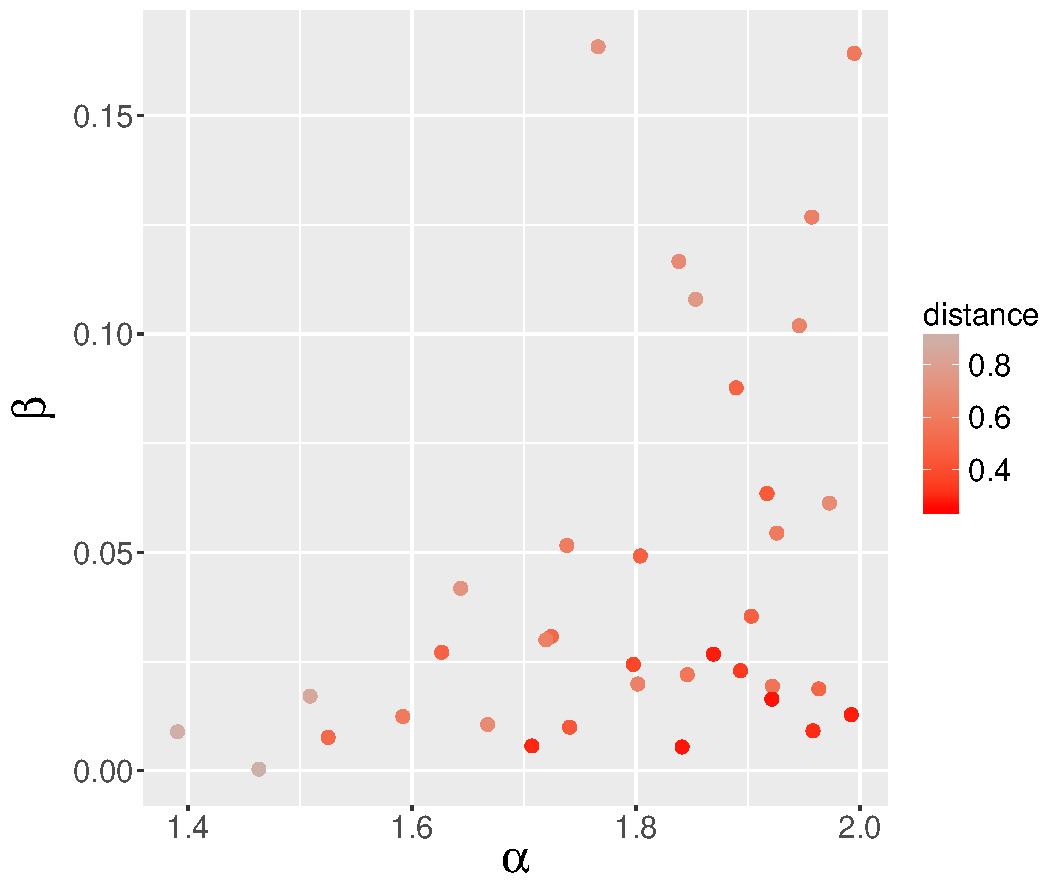
\includegraphics[width=0.48\textwidth]{figures/schelling-relativedistance_metaparams_red}
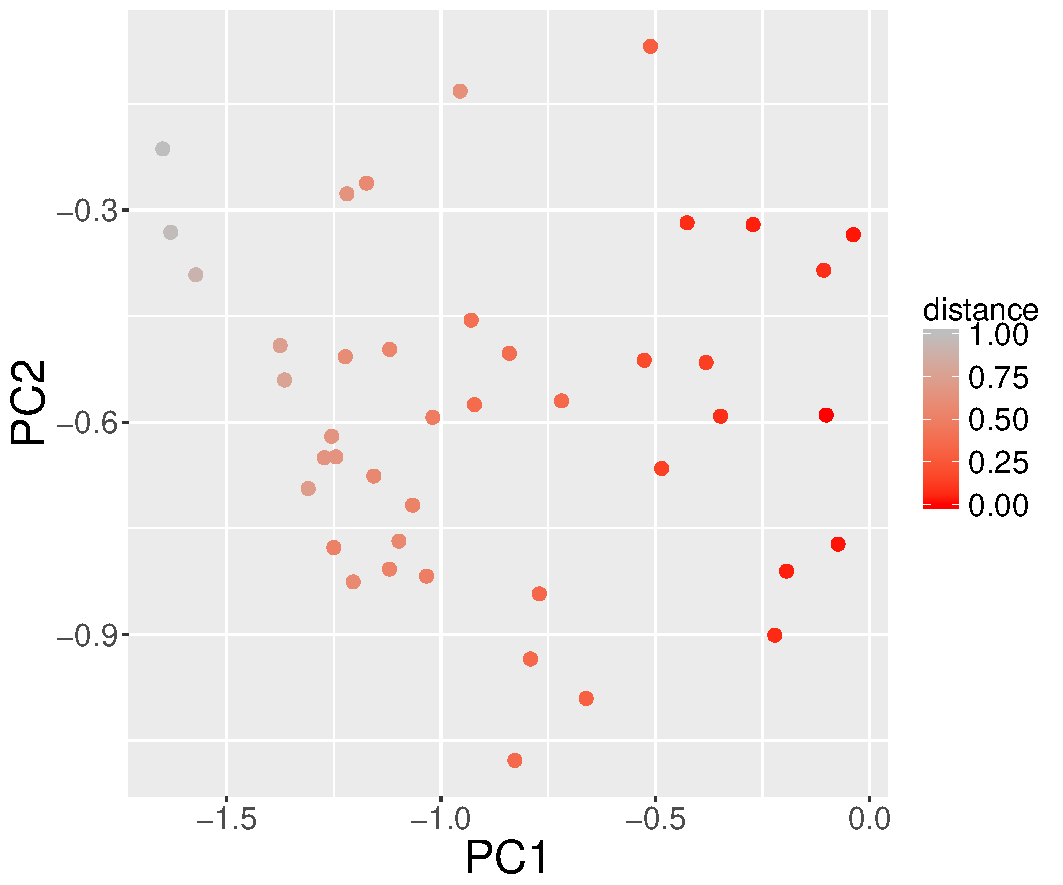
\includegraphics[width=0.48\textwidth]{figures/schelling-relativedistance_morphspace_red}
\caption{\textbf{Relative distances of phase diagrams to the reference across grids for the Schelling model.} Each point corresponds to a spatial configuration and colour gives the relative distance to one of the phase diagrams. We show them in the meta-parameter space (Left) and in the reduced morphological space (Right).\label{fig:schelling-distance-meta}}
\end{figure}
%%%%%%%%%%%%%





\end{document}
